%% LyX 2.1.2 created this file.  For more info, see http://www.lyx.org/.
%% Do not edit unless you really know what you are doing.
\documentclass[UTF8,winfonts]{ctexbook}
\usepackage{mathpazo}
\usepackage[T1]{fontenc}
\usepackage[b5paper]{geometry}
\geometry{verbose,tmargin=2cm,bmargin=2cm,lmargin=2.5cm,rmargin=2cm}
\setcounter{secnumdepth}{3}
\setcounter{tocdepth}{1}
\usepackage{color}
\definecolor{shadecolor}{rgb}{0.835938, 1, 0.863281}
\usepackage{array}
\usepackage{fancybox}
\usepackage{calc}
\usepackage{framed}
\usepackage{url}
\usepackage{graphicx}
\PassOptionsToPackage{normalem}{ulem}
\usepackage{ulem}
\usepackage[unicode=true,pdfusetitle,
 bookmarks=true,bookmarksnumbered=false,bookmarksopen=true,bookmarksopenlevel=1,
 breaklinks=false,pdfborder={0 0 0},backref=false,colorlinks=false]
 {hyperref}

\makeatletter

%%%%%%%%%%%%%%%%%%%%%%%%%%%%%% LyX specific LaTeX commands.
%% Because html converters don't know tabularnewline
\providecommand{\tabularnewline}{\\}

%%%%%%%%%%%%%%%%%%%%%%%%%%%%%% User specified LaTeX commands.
% 如果没有这一句命令,XeTeX会出错,原因参见
% http://bbs.ctex.org/viewthread.php?tid=60547
\DeclareRobustCommand\nobreakspace{\leavevmode\nobreak\ }
\CTEXsetup[number={\thechapter}]{chapter}
\CTEXsetup[format+={\raggedleft}]{chapter}
\CTEXsetup[beforeskip={10pt}]{chapter}
\CTEXsetup[afterskip={30pt}]{chapter}
\def\CTEX@chapter@aftername{\par}
\CTEXsetup[format={\Large\bfseries}]{section}

\makeatother

\begin{document}

\title{中文维基百科概况}


\author{Alexander Misel}

\maketitle

\chapter*{前言}

今天是2016年1月3日,我开始写这本小书。我写这本书的目的是让大家能随着我的介绍,认识真正的维基百科。也希望能够唤醒各位读者对分享知识的追求。我是在2010年8月6日注册维基百科的。但是,和一些用户一样,我在注册前已经在零星地编辑维基百科了。虽然注册已经有了6年,但我真正认识维基百科是从2014年末以后大量参与中文维基百科的工作开始的。

本书的目的就是带大家入门,不光是在维基基础知识上,还包括价值观上。

\bigskip{}


\begin{center}

\includegraphics[scale=0.6]{pic/zhwiki-hans}
\par\end{center}

\tableofcontents{}


\part{了解维基百科}


\chapter{Wiki技术在中文世界的早期传播}

\begin{flushright}
\textit{User:Mountain}%
\footnote{原文位于\href{https://zh.wikibooks.org/wiki/Wiki/\%E5\%8F\%91\%E5\%B1\%95\%E5\%8E\%86\%E5\%8F\%B2}{b:Wiki/发展历史}%
}
\par\end{flushright}


\section{蹒跚起步}

Wiki究竟什么时候最先引入的中文圈子,限于掌握的材料,这是很难彻底探讨清楚的话题。就我们所了解到的情况,在2001年~2002年左右,中文环境里有分散成几群的Wiki实践者,他们各自独立尝试这种新技术。

可查最早的中文Wiki是由索秘软件工作室(Softme Studio)发起WebPM项目的一个子项目jWiki。WebPM项目(Project
Management On Web)的主要目标是为中文自由软件的开发者、使用者和推广者提供基于互联网的开放式管理平台环境。其中jWiki子项目第一阶段开始于2001年12月
27日,结束于2002年01月14日。相关人员告知ID为“浆糊”的网友对这个阶段的贡献最大。第一阶段结束后不久,他们就开设了一个测试的站点softme.org(目前这个站点已经废弃),来测试他们的Wiki系统。WebPM项目的开发团队还是中文环境里面比较早实践XP的队伍。jWiki项目在2004年依然活跃,曾经发布了jWiki-v2.0.1的版本。

2002年5月份,中蟒大杂院开通。中蟒大杂院是一个修改过的基于MoinMoin的Wiki系统,它服务于中蟒计划。中蟒是一种基于Python2.1.3
版的中文编程语言,除了保留字,变量名称可用中文外,很多内建的数据类型也都是用中文来表示的。目前中蟒计划已不再维护,而中蟒大杂院在2006年之后也已经鲜有人编辑了。中蟒大杂院的讨论主要集中在Python的技术方面,而对Wiki自身的讨论比较少。2002年10月,中文维基百科开始正式起步,它是到目前为止中文圈中最大的Wiki站点之一。2002年11月初,贸大Wiki开通,它是对外经济贸易大学的校园Wiki网站,但如今也已经废弃不用了。


\section{在网志空间的传播}

如果说2001年~2002年大家都还在工具上作研究,经过一年左右的实践和学习,2003年~2004年大家开始发出自己的声音,阐释自己对Wiki的理解。而同时,在中文环境里Blog也开始兴起,Blog为Wiki的传播提供了全新的途径。

其实早在2002年底,中文Blog的先行者cnblog.org就开始了关于Wiki的探讨。2002年11月22日峨桥的主人goghs发了一篇介绍Wiki的文章《Wiki/Wakka/Blog
– 一点浅见》,他对Wiki的理解已经相当深刻了——

\noindent \begin{center}
\doublebox{\begin{minipage}[t]{0.7\columnwidth}%
\textit{“Wiki站点一般都有着一个严格的共同关注,Wiki的主体一般是明确的坚定的。Wiki站点的内容要求着高度相关性。最其确定的主旨,任何写作者和参与者都应当严肃地遵从。Wiki的协作是针对同一主题作外延式和内涵式的扩展,将同一个问题谈得很充分很深入。Wiki非常适合于做一种
“All about something”的站点。个性化在这里不是最重要的,信息的完整性和充分性以及权威性才是真正的目标。Wiki由于其技术实现和含义的交织和复杂性,如果你漫无主题地去发挥,最终连建立者自己都会很快的迷失。Wiki使用最多也最合适的就是去共同进行文档的写作或者文章/书籍的写作。特别是技术相关的(尤以程序开发相关的)FAQ,更多的也是更合适地以Wiki来展现。”}%
\end{minipage}}
\par\end{center}

贸大Wiki撰文探讨Wiki的开放性,并且也幽默的贴出了“一个民有,民治,民享的Wiki将永存于世!”的口号,互联网早期的理想在这里回荡。2003年9月5日,台湾的自由软体铸造场计划网站发表了《名家专访:Blog
与 Wiki 的对话》,专门探讨Blog与Wiki。

2003年~2004年也是维基百科迅速成长的时期,敏感的网友开始对这个计划表示关注。2004年6月初cnblog.org上Eric
Nash《关于wiki的一些联想》引起了不少人的关注。Eric Nash从自己使用Google和Wikipedia的搜索习惯谈起,认为Wiki的庞大访问量和长时效的特点会弥补它在准确与权威上的问题,又从信息组织方式的有序与无序的角度探讨Wiki和搜索引擎的不同,最后他得出这样的结论:

\noindent \begin{center}
\doublebox{\begin{minipage}[t]{0.7\columnwidth}%
\textit{“web是一个通过Link连起来的杂乱无章的世界,wiki的无非是人们在无序中寻求次序的本能需要,一个理想的web应该是杂乱无章无序世界加上一个有序的庞大的wiki的有序世界,这两个相反的世界在web上又是共生共容,就相当与太极图上的黑白两个半圆——到最好总是那么简单和谐。”}%
\end{minipage}}
\par\end{center}

在这篇文章引发的讨论里,网友maomy的评论至今值得我们思考:

\noindent \begin{center}
\doublebox{\begin{minipage}[t]{0.7\columnwidth}%
\textit{“但是有一个问题,wiki对任何人的可写性,可能导致你今天刚写上去的内容就被人涂改了,甚至改的观点完全不同——这还不包括恶意破坏,或者因强烈的观点冲突而删除你的原文重写的可能。理想的状态当然是每个人都足够认真严肃地去写wiki,但即便如此,也不能保证我们能信任wiki中的大多数信息,因为我们都知道人的偏见和狭隘是多么难于克服。更何况,这种理想状态的达到都是非常困难的。”}%
\end{minipage}}
\par\end{center}

中文早期的Blog写手Zheng也撰文探讨Wiki无穷尽的生成能力和蔑视时间变化的特性。

\noindent \begin{center}
\begin{framed}%
\textit{“如何才是Wiki区别于其他Web应用的不同之处呢?应该是如下两点?}

\textit{1、无穷尽的网页自动生成功能:Wiki创建页面的方式一直让我很着迷。对其他文档处理程序来说,可以通过创建命令来创建出很多很多的文档,但是文档之间并没有彼此的联系,它们就像散沙。可是Wiki不同,它不用特别的创建命令,在人们需要的地方,它就能够自动生成,并且所成的页面和原来的页面存在一个由词构成的联结点。人们可以在Wiki上无限制的创建出新的页面,而这些页面,无论它们相距多远,总存在千丝万缕的联系。它们是一个整体。是一个不断的、没有终结的在扩展的书。这种扩展无处不在,任何一个缝隙都能成为一个无穷尽迷宫的入点。它没有距离、没有空间,但却有无穷尽的可能出现。它像不像人们所拥有的知识本身?像不像人们海阔天空的联想本身?}

\textit{2、它超出时间之外,也就是它是可逆的:这实际上来源于Wiki的版本记录和恢复功能。和其他文档处理程序不同,Wiki把过程也作为他重点处理的对象和最终的文本地位一样。所有的变化都被记录,能够任意恢复到变化前的某一点。从这方面来说,时间对它无效。从前台看,它一直向前,但是在后台,所有的历史、所有的数据都被保存。这是一个经典物理世界和现实世界的奇妙变异体。一方面,谁也无法预知它的未来,另一方面,却可以回到过去。作为一个对比,人的状态可以被记录,但老去是不可逆的。
Wiki却可以。那是否意味着,Wiki的独特之处在于对空间无穷尽的深刻理解和对时间的蔑视?”}\end{framed}
\par\end{center}

The Way We Web是中国大陆一位有影响的Blogger,他在2005年1月18日写了一篇blog—《WIKI,感觉不仅仅是百科全书》,其中有一段这样说的:

“百科全书试图将词条定义为某种相对静止从而可以把握的东西,而WIKI不一样,它既将这种相对的静止抽象出来,也记录了这一静止后面的流动不居的书写过程,这二者的共存使人明白:历史无定论,任何东西都没有定论,历史就是我们书写时应该保持谦卑的那位主人。”

所有这些吉光片羽式的小小讨论片段都给读者留下了很深的印象。


\section{中文维基百科}

2002年10月,中文维基百科创建。在完成了基本的界面汉化之后,除了撰写文章,早期的参与者也把很多精力放到了移植英文版的各种政策之上,而这些政策体现了维基百科社群对Wiki的认知。

Formulax在2003年3月20日将英文版NPOV最初的翻译贴上来,这就是维基百科的基础政策之一—中立的观点。

对“共识”这个概念的首次讨论来源于2003年底对“理想语”争论。一个用户反复张贴自己原创的、却又无法令别人解读的“理想语”条目,这在社群内部引发了不小的争议,最终这个条目被删除。但在争论过程之中,社群觉得有必要建立一个政策产生的机制,Dersonlwd创建了页面决议产生的程序,而Lorenzarius在讨论中第一次提到了“共识”这个概念。

\noindent \begin{center}
\doublebox{\begin{minipage}[t]{0.7\columnwidth}%
\textit{\textquotedbl{}Wikipedia一般都是采用consensus来决定事情的(而不是投票!!!Tyranny
of the majority)。而且正如Formulax所说,在这里每个人都是平等的,这正是Wiki的精神!不要把管理员当作是elite!……
Consensus追求的是达致一个所有人都可以接受的合理性的决定,以尝试照顾所有人的意见。如果每人都执着自己的想法,不去聆听别人的意见,即使强行下了个决定,总会有一方会不开心。所以我认为投票是一种非常差的决议形式,虽然它是很快,但它强行把所有人分到不同的类别中(但事实上人的意见不是如此壁垒分明的,而应该是像一个spectrum一样),造成分化和对立,而这与Wiki的协作精神相差太远了。\textquotedbl{}}%
\end{minipage}}
\par\end{center}


\subsection{传统媒体的关注}

2003年10月《中国电脑教育报》发表了作者布衣蝶的文章《我也来写百科全书》,这是中文媒体第一次介绍维基百科。

2004年2、3月间大陆主流媒体开始了对维基百科的报道。2004年2月15日《新周刊》在第173期发表了记者蒋亦凡的报道《知识狂欢时代的自由百科》,这是中文媒体第一次以中文维基百科为主题的新闻报道。2月29日上海《星期日新闻晨报》第16版发表了记者刘迪关于维基百科的报道。

2004年2月26日《三联生活周刊·总275期》,记者尚进对Wiki作了长篇报道。这篇编译过来的报道,其中有对Ward Cunningham的专访,所涉及的内容非常深入,在当时颇有影响。

2004年3月16日《中国青年报》登刊了记者周欣宇关于维基百科的文章《维基百科:分享知识的新方式》。紧接着《新京报》报道记者周文翰的文章《自由知识革命从自由百科全书开始》。3月23日《南方都市报》报道了维基百科:《维基百科:互动的乌托邦?》。

2004年5月10日《新京报》报道:维基百科获得电子艺术大奖。其后,又有两家台湾主流媒体也报道了维基百科:5月16日台湾《中时晚报》第4版刊登了《维基网络百科:大家来写百科全书》专题,是台湾主流媒体第一次以显著版面介绍维基百科。6月台湾联合报报道了记者陈宛茜的文章《Wiki百科网书,你也可写一笔》。

一个有趣的问题是,计算机技术的专业媒体非常忽视非商业性质的Wiki技术,而中国大陆比较新锐的传统媒体却对Wiki技术和维基百科给予了相当的关注。


\chapter{我是一个新手}

虽然我已经不再称自己是新手了,但是我并不了解维基百科的方方面面,但我会把我认为新手需要知道的事情在这里讲出来。虽然维基社群里也有相应的页面,但是其实如果是一本书的话,我想大家会更愿意看一些。

很多新手都不知道怎么入门,而其实维基百科就有现成的入门宝典。如果你问一个维基人新手入门的指南在哪儿,他也许会直接抛给你一串字符:

\noindent \begin{center}
\ovalbox{\begin{minipage}[t]{0.2\columnwidth}%
\begin{center}
\textbf{\textcolor{blue}{WP:}}\textbf{\textcolor{magenta}{入门}}
\par\end{center}%
\end{minipage}}
\par\end{center}

实话讲,在我还是新手的时候,也和你一样一头雾水。如果让我给一个新手解释这串字符是干什么的,我会让他直接在搜索框搜索这串字符。但这里我多讲一点。蓝色的WP是Wikipedia的缩略,是维基百科名字空间,英文冒号是限定符。名字空间自然是要区分各种页面的。不写名字空间的页面都位于条目名字空间。后面的“入门”二字才叫做页面名称。前后结合起来就确定了这个页面——Wikipedia:入门。

有人可能想问,为什么真正到达的页面名称是“维基百科:新手入门/主页”。%
\footnote{\href{https://zh.wikipedia.org/wiki/Wikipedia:新手入門/主頁}{https://zh.wikipedia.org/wiki/Wikipedia:新手入門/主頁}%
}其实,这是后面还会提到的重定向功能,顾名思义,就是从一个页面自动跳转到另一个页面的。

接下来我将按照新手入门中的顺序给读者朋友们介绍。这里我不会照抄新手入门中的内容,但你需要知道虽然我可能不会把新手入门全部内容都提到,但是建议新手有时间是要全部看完。


\section{维基百科介绍}

维基百科是一部网上百科全书,有很多与其他百科全书不同的特点,在编写时也有一些值得留意的地方。

\noindent \begin{center}
\doublebox{\begin{minipage}[t]{0.7\columnwidth}%
\textit{百科全书是概要介绍人类的全部知识或某一类知识的工具书。按照辞典形式编排,以条目为基本单元,收集各知识领域的名词、熟语、地名、事件、人物、著作等等,但不收录词语,故不同于语文辞典。}

\begin{flushright}
\textit{——源自“百科全书”条目}
\par\end{flushright}%
\end{minipage}}
\par\end{center}

本节进一步介绍一些维基百科的细节以及一些术语的意思。


\subsection{谁在写维基百科}

维基百科由来自全世界的维基人协同写作。无数人为维基百科做出了贡献。所有的人都可以对维基百科做出修改。您只需知道如何编辑页面。维基百科的运作者是\textbf{维基媒体基金会}%
\footnote{维基媒体基金会(英语:Wikimedia Foundation,WMF)是美国的一个非盈利慈善组织,其总部设在加利福尼亚州旧金山,运转多个Wiki项目。参见\href{https://zh.wikipedia.org/wiki/\%E7\%BB\%B4\%E5\%9F\%BA\%E5\%AA\%92\%E4\%BD\%93\%E5\%9F\%BA\%E9\%87\%91\%E4\%BC\%9A}{维基媒体基金会}条目。%
},但该组织不直接负责编写维基百科。


\subsection{维基百科收录什么呢}

维基百科是一部百科全书。它没有条目数量限制,凡是一切具有\textbf{关注度}%
\footnote{关于在维基百科中\textbf{关注度}指的是什么,请参考后文。%
}且能获得查证的事物,都可以写成维基百科条目。维基介绍页面下面会告诉大家维基百科\textbf{\emph{不是}}下面这些

\noindent \begin{center}
\begin{minipage}[t]{0.7\columnwidth}%
\begin{shaded}%
辞典、发表个人观点的地方、宣传工具、原始数据收集处、个人空间、问题集、主题关系松散的数据库或列表、旅游指南、悼词、新闻报道、宗谱、电话簿条目、黄页、说明书、游戏攻略及虚构作品情节的介绍\end{shaded}%
\end{minipage}
\par\end{center}

我们亦\textbf{\emph{不是}}预言家。所有关于将来会发生的条目都必须可以证实,而这些将来事件成为过去后,都必须有值得记载的价值。


\subsection{维基百科的版权}

维基百科的所有内容依照知识共享 署名-相同方式共享 3.0协议(CC BY-SA 3.0)%
\footnote{维基百科上的CC BY-SA 3.0协议未本地化版本文本,见于\href{https://zh.wikipedia.org/wiki/Wikipedia:CC_BY-SA_3.0\%E5\%8D\%8F\%E8\%AE\%AE\%E6\%96\%87\%E6\%9C\%AC}{WP:CC}。%
}公开发布。这看起来似乎有些复杂,简而言之:任何人都可以自由查看、复制、修改和使用您编写的内容(包括商业用途),而无需得到您的同意。但是他们需要标注您的用户名作为署名,并使用同一个许可协议发布,这确保了所有后续修改均是自由开放的。

互联网上的绝大多数内容均不能直接复制至维基百科。人们所写的东西大多都有著作权,维基百科不能未经允许而随便转载这些内容,未经允许而随便转载是违法行为。版权法保护的是思想的表现形式(比如一段介绍“相对论”的文字叙述),而不是思想本身(比如相对论本身这一理论)。您只需要用自己的话把它重新写下来,或者自己拍摄照片,便能避免任何侵犯著作权的问题。


\subsection{一些术语的意思}
\begin{description}
\item [{条目}] 在一些网上百科全书中也称“词条”,指所有的“百科全书文章”,以及目录索引(例如列表,年表等)。条目是百科全书的最基本单元,是知识和信息的集成载体单元。一篇优秀的条目拥有一个特定的百科全书主题,并对主题进行了全面的摘要性总结,同时有对可靠来源的引用。维基百科中的条目也包括了关系紧密的相关主题的列表索引,并且相关主题之间通过链接产生关联。
\item [{社群}] 维基百科社区由维基人组成,会就维基百科各项内容进行讨论(在\textbf{互助客栈}%
\footnote{互助客栈的链接:\href{https://zh.wikipedia.org/wiki/Wikipedia:\%E4\%BA\%92\%E5\%8A\%A9\%E5\%AE\%A2\%E6\%A0\%88}{WP:VP},后文还会说到互助客栈。%
}),并尝试改善维基百科。您也可以参与讨论。
\item [{维基人}] 全称维基百科人,指所有参与维基协作项目的人,无论其贡献多少。
\item [{管理员}] 管理员可以删除、保护条目,也可以授予其他用户权限。请注意,管理员不能直接修改维基百科的运行程序。
\end{description}
更多维基百科术语,可以参见维基百科中的术语表(\href{https://zh.wikipedia.org/wiki/Wikipedia:\%E6\%9C\%AF\%E8\%AF\%AD\%E8\%A1\%A8}{WP:G})。


\section{探索维基}


\subsection{浏览维基百科}

您可以选择多种方式来浏览维基百科:
\begin{itemize}
\item 文章中的蓝色文字是内部链接,只要点击就可以转到相应页面。
\item 屏幕右上角是一个搜索框,在搜索框中输入关键词,按下回车键就可以得到结果。若需要更详细的帮助,可以看搜索帮助学习如何搜索。
\item 浏览我们的主题首页或分类索引,从中点击任何您感兴趣的内容。
\item 查看我们的特色内容,它们可以视为维基百科条目写作的典范。
\item 点击页面左边导航栏的“随机页面”连接,将随机打开到一个条目。
\item 从首页展示的特色或优良作品开始,探索维基百科。
\end{itemize}

\subsection{访问维基百科}

对于港澳台以及海外,访问中文维基百科通常是不会出现问题的。由于经常有各种镜像网站,需要指出中文维基百科的网址为:
\begin{itemize}
\item 桌面版:\texttt{https://zh.wikipedia.org}
\item 移动版%
\footnote{咦,怎么是“移动”版?其实,这里的“移动”非中国移动,而是mobile的意思,也就是手机版。%
}:\texttt{https://zh.m.wikipedia.org}
\end{itemize}
对于中国大陆的维基百科使用者,常常会面临因政府审查而难以访问维基百科。目前来说既能\texttt{\emph{阅读}}又能\texttt{\emph{注册编辑}}维基百科的方法主要是两类:

\begin{center}
\begin{tabular}{|c|>{\centering}p{7cm}|}
\hline 
方法 & 描述\tabularnewline
\hline 
\hline 
VPN+IP封禁豁免权(ipbe) & VPN虽然方便,但需要进行邮件申请ipbe权才能编辑\tabularnewline
\hline 
hosts/DNS加密软件 & hosts稳定无副作用,DNS加密软件如果是全局的会影响一些国内网站的访问速度\tabularnewline
\hline 
\end{tabular}
\par\end{center}

维基百科亦推出了官方的iOS、Android和Windows 8应用程序。这些程序均可以通过相应的应用商店下载。


\section{编辑入门}

不要害怕编辑,勇于更新页面!维基百科上几乎所有的页面都可以编辑。只要点击页面上方的“编辑”按钮,就可以编辑你正在浏览的页面。这是维基百科的基本功能之一。如果你看到的是“查看源代码”按钮而不是“编辑”按钮,则表示页面受到了保护。页面被保护原因除了防止破坏,亦有可能因为行政原因。不过,维基百科上绝大多数页面均允许编辑。

你可以查找可以改善的任何东西,不论是内容、文容或编排方面的,然后更正它。放心,维基百科保存了过往编辑版本,错误的修订很轻易就能被取消或改善。当你向维基百科增添内容的时候,请务必列明来源,无法查证的内容可能会被移除。

要想练习编辑,请前往维基百科:沙盒(\href{https://zh.wikipedia.org/wiki/Wikipedia:\%E6\%B2\%99\%E7\%9B\%92}{WP:SB})。点击“编辑”按钮,将会出现一个大的、白色的文本框(称作编辑框),位于编辑窗口的中部。向编辑框中键入任何你感兴趣的内容,或者修改别人写下的东西。然后点击“保存编辑”按钮,欣赏你第一次编辑的成果吧!在沙盒中你可以尽情练习你所学到的一切,而不会对维基百科造成破坏。


\subsection{显示预览}

\begin{figure}[h]
\begin{centering}
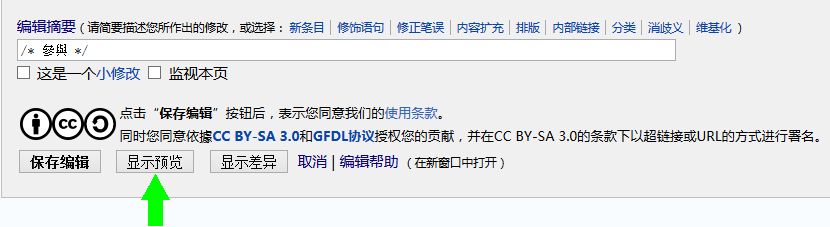
\includegraphics[scale=0.5]{pic/Show_preview}
\par\end{centering}

\protect\caption{“显示预览”按钮位于编辑摘要框下面,保存按钮右边。}


\end{figure}


在编辑操作中,最重要的一步是进行预览——看看页面将会显示成什么样。此外“显示更改”按钮可以显示你编辑之前及之后的差异。

我们建议你养成每次编辑都预览的好习惯,因为人人都可能会犯错误,无论新手或老手均是如此。若你发现预览的结果有问题,或者没出现你想要的内容,则请检查编辑框中的代码并更正。如果无问题,就可以点击“保存编辑”来保存条目。


\subsection{编辑摘要}

编辑完毕之后,最好在编辑摘要框中写出你这次编辑的目的、修改了的内容等等。写只需要花费你几秒钟的时间,但却能节省其他编辑很多时间。当然,这项不是强制性的。

为了简便起见,你亦可以直接点击系统提供的选项。例如,你更正了一个拼写错误,则可以选择“修正笔误”。如果你只做了小修改,则可以勾选“这是一个小修改”框。


\subsection{保存页面}

是否已经写了编辑摘要?并且预览了页面? 那么你就可以点击“保存编辑”,完成页面的编辑过程。修改一旦被保存,即依有关授权协议发布,并且永久存放在维基百科服务器上,供任何人士查阅。

下一环节,将会介绍各个维基代码所代表的内容。


\subsection{维基文本}

\textbf{提示}:新的简易编辑方式--可视化编辑器已经向注册用户开放。用户只需于登入,并在\textbf{参数设置}%
\footnote{参数设置就位于页面桌面版的右上角。也可以使用\href{https://zh.wikipedia.org/wiki/Special:\%E5\%8F\%82\%E6\%95\%B0\%E8\%AE\%BE\%E7\%BD\%AE}{Special:参数设置}访问。%
}中启用即可。启用后,编辑条目或用户页时,页顶的“编辑”链接将链接至可视化编辑器界面,从此不再需要学习下列的维基代码!然而,该编辑器目前尚处于测试阶段,部分功能尚未完善且可能会出错,\textbf{请小心使用}!(更详细的编辑帮助见于\href{https://zh.wikipedia.org/wiki/Help:\%E7\%BC\%96\%E8\%BE\%91\%E9\%A1\%B5\%E9\%9D\%A2}{Help:EDIT})

掌握简单的维基文本之后,就能看懂源代码编辑时各种条目格式表示方法的含义了。如果不熟,可以查询备忘单(\href{https://zh.wikipedia.org/wiki/Wikipedia:\%E5\%82\%99\%E5\%BF\%98\%E5\%96\%AE}{WP:CHEAT})。


\subsection{格式指南}

维基百科有一套格式指引,未能合乎这些指引的页面则需要\textbf{维基化}%
\footnote{何为“维基化”?\textbf{维基化}(Wikify)是将内容修正为符合维基百科:格式手册标准的过程。%
}。

以下就各项格式作出介绍,有关各项格式的详情则请参考格式手册(\href{https://zh.wikipedia.org/wiki/Wikipedia:\%E6\%A0\%BC\%E5\%BC\%8F\%E6\%89\%8B\%E5\%86\%8C}{WP:MOS})。网页上比较长,其实概括起来就几句话:

\begin{center}
\begin{minipage}[t]{0.7\columnwidth}%
\begin{shaded}%
每一个名称在第一次出现时都要以\textbf{粗体}显示。使用全角\textbf{标点}符号。中文都应该优先提及,有需要再用\textbf{外文}。尽可能在首句带出文章所属的\textbf{主题}。\textbf{历史}上的概念应注明有效时间。\textbf{日期}一般应使公元纪年,不要简写。\textbf{度量衡}一般应采用国际单位制。在中文语境内,字与字之间应该不留\textbf{空格}。\textbf{外部链接}放于条目最后,不可过多。格式代码不太花俏。\end{shaded}%
\end{minipage}
\par\end{center}


\subsubsection{特定主题指引}

格式手册的目的很简单:让格式整齐统一。以下规则并非金科玉律。许多种格式并无高下之分,但如果每人都遵循同一格式,维基百科将更为易读易用,当然也更易撰写编辑。

新手应注意,清晰、丰富,中立的原则比之格式更为重要。\textbf{撰写者没有义务遵循以下规则,这些规则仅作为推荐使用:}编辑的乐趣在于不必达到完美。

其他维基参与者会在编辑维基百科的时候,会按照这个指引修正不规范格式的条目,条目会渐渐的符合指引内容。


\section{方针指引}

维基百科上有数类内容,分为正式方针、英语维基方针、正式指引、英语维基指引、格式指南(上页提及的)、英语维基格式指南(上页亦有提及)、论述、维基专题、基金会决议制度等。


\subsection{制定}

维基百科方针主要是取得\textbf{共识}%
\footnote{\textbf{共识}是维基百科编者作出决议的第一途径。参见\href{https://zh.wikipedia.org/wiki/Wikipedia:\%E5\%85\%B1\%E8\%AF\%86}{WP:CON}。%
}来制定的。这些共识可以透过对复杂难题的公开辩论,也可从既有惯例简单发展而出。在大多数情况,被人们接受的标准并不是立即就正式地写下来。因此,本页及其他页面上有关维基百科方针的叙述,是用来描述那些经长期发展而成的既有社群准则。

总体来讲,有三种方式使某项方针成为正式:
\begin{itemize}
\item 由吉米·威尔士(Jimmy Wales)或维基媒体理事会(Wikimedia Board)制定及颁布。
\item 一项提案经讨论取得共识后被正式采用。
\item 逐渐演化出的常规或惯例。将方针正式化的观点已在互助客栈、邮件列表、以及相关的条目对话页上彰著广告,持续合理的时间,并且所有的反对意见都已经妥善处理。
\end{itemize}

\subsection{五大支柱}

五大支柱决定维基百科发展方向,亦为众方针及指引之基础,故尤其重要。
\begin{description}
\item [{维基百科是一部百科全书}] 参见前文介绍的维基百科不是什么(\href{https://zh.wikipedia.org/wiki/Wikipedia:\%E7\%BB\%B4\%E5\%9F\%BA\%E7\%99\%BE\%E7\%A7\%91\%E4\%B8\%8D\%E6\%98\%AF\%E4\%BB\%80\%E4\%B9\%88}{WP:NOT})。
\item [{维基百科采用中立观点}] 所有维基百科条目以及其他百科式内容必须以中立的观点书写,平等、成比例且不带偏见地表达重要的观点。非中立的条目应当挂上\texttt{\{\{npov\}\}}模板并进行编辑,移除任何不适当内容。参见\href{https://zh.wikipedia.org/wiki/Wikipedia:\%E4\%B8\%AD\%E7\%AB\%8B\%E7\%9A\%84\%E8\%A7\%82\%E7\%82\%B9}{WP:NPOV}。
\item [{维基百科是版权开放的}] 维基百科正式的版权宣告参见\href{https://zh.wikipedia.org/wiki/Wikipedia:\%E7\%89\%88\%E6\%9D\%83\%E4\%BF\%A1\%E6\%81\%AF}{WP:C}。
\item [{维基人以礼相待、相互尊重}] 维基百科的参与者来自不同的国家和地区,拥有着不同的文化。我们有着不同的观点、看法和背景,有些时候非常多样。尊重他人是建设这部百科全书的有效合作关键。参见\href{https://zh.wikipedia.org/wiki/Wikipedia:\%E7\%A4\%BC\%E4\%BB\%AA}{WP:EQ}。
\item [{维基百科不墨守成规}] 如果有规则妨碍你改进或维护维基百科,请忽略该规则,这五大支柱除外。必要时请去互助客栈讨论。参见\href{https://zh.wikipedia.org/wiki/Wikipedia:\%E5\%BF\%BD\%E7\%95\%A5\%E6\%89\%80\%E6\%9C\%89\%E8\%A7\%84\%E5\%88\%99}{WP:IAR}。
\end{description}

\subsection{基金会方针}

由创办维基百科的维基媒体基金会颁布的方针,必须遵守,并凌驾于本地方针之上。
\begin{description}
\item [{基金会行动}] 维基媒体基金会偶尔会在未得到社群共识支持的情况下删除、保护或清空一个页面,此等暂举乃用以解决法律问题及阻止人身攻击,任何用户均不应回退该等操作。
\item [{用户查核}] 只有在合乎维基媒体基金会的隐私方针并在合理怀疑下方可启动机制查核用户所使用的IP地址,查核之后亦只能给出有没有傀儡等信息,不能给出详细信息。
\end{description}

\subsection{方针与指引总览}

维基百科上的方针是每个参与者都必须遵守的要求,违反者轻则警告或提醒,重则可能会被禁止编辑。维基百科的方针和指引构成了一个体系,保证了维基百科的正常运行。维基百科的方针指引体系概要如下

\begin{center}
\begin{tabular}{|c|>{\raggedright}p{9cm}|}
\hline 
类别 & 广泛、基本的方针和指引\tabularnewline
\hline 
\hline 
 & 忽略所有规则\tabularnewline
\hline 
内容方针 & 维基百科不是什么 – 中立的观点 – 可供查证 – 非原创研究\tabularnewline
\hline 
内容指引 & 列明来源 – 不要制造恶作剧 – 不要包含原始资料的副本 –  可靠来源 – 胡言乱语\tabularnewline
\hline 
编辑指引 & 条目长度 – 勇于更新页面 – 页面分类 – 消歧义 – 行话解释 – 小作品 – 摘要格式\tabularnewline
\hline 
关注度指引 & 关注度\tabularnewline
\hline 
命名常规 & 命名常规 – 页面分类\tabularnewline
\hline 
格式指引 & 格式手册\tabularnewline
\hline 
行为准则 & 文明 – 共识 – 编辑守则 – 骚扰 – 破坏\tabularnewline
\hline 
态度指引 & 善意推定 – 利益冲突 – 扰乱性编辑 – 礼仪 – 讨论页指导\tabularnewline
\hline 
删除方针 & 删除方针 – 快速删除方针\tabularnewline
\hline 
删除指引 & 删除程序\tabularnewline
\hline 
程序性方针 & 方针与指引\tabularnewline
\hline 
强制执行方针 & 管理员 – 封禁方针 – 保护方针\tabularnewline
\hline 
法律方针 & 著作权信息 – 不要诉诸法律威胁 – 使用条款\tabularnewline
\hline 
项目内容指引 & 用户页\tabularnewline
\hline 
\end{tabular}
\par\end{center}


\subsection{常用方针解读}
\begin{description}
\item [{非原创研究}] 维基百科不是发表原创研究或原创观念的场所。所谓原创研究或原创观念,指的是未发表的事实、争论、推论和想法;以及对已发表材料进行的未发表分析或总结,并产生了新的立场。(\href{https://zh.wikipedia.org/wiki/Wikipedia:\%E9\%9D\%9E\%E5\%8E\%9F\%E5\%88\%9B\%E7\%A0\%94\%E7\%A9\%B6}{WP:NOR})
\item [{可供查证}] 被质疑或可能被质疑的材料,以及所有的引言,都应带有可靠、公开的来源。
\item [{共识}] 各项讨论、方针的结果均出于此。
\item [{快速删除的标准}] 在合乎指定要求,条目可以不经讨论被删除。
\item [{文件使用守则}] 使用文件的要求。
\item [{不要人身攻击}] 要针对文章内容发表意见,而非针对文章贡献者(这是“对事不对人”的原则)。所有人身攻击将会被移除甚或删除,严重者则封禁处理。
\item [{删除守则}] 一般来说,只有新建的错误页面(例如一段随便输入的文字)才会被删除,另外,如果一篇文章全部侵犯了版权,经过确认后也会被删除。我们应该尽量保留所有合乎百科全书条目的文章,删除投票应该是最后的选择。
\item [{回退不过三原则}] 不要在24小时之内回退任何单独的页面超过三次,这不包括自己回退或对简单破坏的纠正。违者查封24小时,再犯者加重。
\end{description}

\subsection{常用指引解读}
\begin{description}
\item [{关注度}] 维基百科收录“值得关注的主题”,亦即已被独立来源在相当程度上予以关注的主题。如果一个没有违反“维基百科不是什么”的主题,得到了可靠的第二手来源的有效介绍,我们便可假定该主题符合独立条目的收录标准。关注度并不直接影响条目内容,而只决定其存在与否。
\item [{可靠来源}] 维基百科的条目应该采纳可靠的已经出版的来源。使得大多数人的意见和重要的少数意见被收录。
\item [{页面分类}] 页面分类能帮助用户通过分类检索维基百科。
\item 
\end{description}

\section{交流讨论}

与其它百科类网站类似的是,维基百科有其专属的用户页面及沟通页面。另外,多人沟通可前往互助客栈留言。若是针对单个条目的讨论,可在条目的讨论页交流。而这三者都是基于MediaWiki程序自身的讨论页设计的。

讨论页是维基百科页面的一种,它包含了所有对主题文章的讨论。要查看讨论页,只要点击页面旁的“讨论”链接即可。当你在讨论页时,你可以用“条目”(如果不是条目,则可能是其他相应名称,比如“项目页面”等)链接返回到该讨论页所讨论的文章。

讨论页的主要目的是从一种百科全书的观点来协助撰写更好的相关文章。任何的问题、疑虑、怀疑、参考文献、有关文章的论战或者评论都可以在相关的讨论页提出来。

讨论页是用来帮助编写条目的,而不是进行广告或测试的场所,亦非该条目主题的论坛或讨论区。虽然有讨论页,但亦请认真提交编写的条目。


\subsection{用户讨论页}

您的用户页有一个讨论页(对话页),它的功能有所不同。在您的用户名和地址旁会有一个到您讨论页的链接。如果有人在您的讨论页做了修改或加入了内容,您会看到“您有新消息”出现在页面的顶部,你也可以选择收取电子邮件通知。这些讨论页可以用来作为与其他人的联络和沟通。但要注意的是讨论页是公开的,如果您需要私下与其他人联系,请使用电子邮件或IM。

要到用户的讨论页,只要先到该用户的页面,然后点击页面旁的“讨论”即可。在“最近更新”、“监视列表”页面中,您可以直接点击括号内的链接到用户讨论页。


\subsection{互助客栈}

互助客栈是讨论页的一种形式,其功能近乎于论坛,但需要特别注意的是,互助客栈\textbf{不是论坛}。

你可以在维基百科每一个页面的左侧的“帮助”菜单下找到到互助客栈的快捷方式。进入后请选择适当的版面提出问题。


\subsection{一句话}

请善用讨论页作理性、有意议、有建议性的讨论。


\section{用户权限}


\subsection{被封禁用户}

所有被封禁用户都不能编辑维基百科,但能够阅读。封禁主要用作避免维基百科受到破坏,或减低潜在问题发生的机会,且应是阻止上述问题的最后手段。如果他们对于封禁有异议,可以通过用户讨论页或电子邮件提出申诉。


\subsection{匿名用户}

没有注册账号或登录的用户是以他们的IP地址作为识别。他们能够阅读维基百科的所有页面(除了部分要求特定权限的特殊页面),可以编辑已被保护以外的页面,亦可以创建页面,只需要在搜寻栏输入欲撰写条目的名称,或者点击条目中的红字连结,便可进入编辑新条目的页面,但在创建维基百科的某些部分时可能需要请求帮助(例如被白纸保护的页面)。他们不能上传文件和图片。如果他们想编辑一个或更多的外部链接或注册一个账号时,必须通过验证码。他们通常只有用户讨论页,而没有用户页。


\subsection{注册用户}

注册用户是指拥有一个维基百科账号的人。注册成为维基百科的用户,不仅过程快捷、免费及方便,更可享有一些非注册用户没有的权限,而注册并不要求提供个人资料(电邮地址为选填项目)。


\subsection{自动确认用户}

\textbf{自动确认用户}是维基百科用户的一种。在中文维基百科,任何注册达7天并编辑达50次的用户,均会成为自动确认用户。在善意假定的原则下,我们假定取得自动确认用户权限的新用户,都不会是只为破坏而注册的账号,或者是由他人控制的傀儡账号。我们亦假定该等用户已在维基百科累积一定的经验,并对维基百科运作有一定的认识。因此,自动确认用户可享有一些非自动确认用户没有的权限。


\subsection{其他权限}
\begin{description}
\item [{IP封禁例外}] 如果您有必要使用代理服务器(例如Tor)作出编辑或您所用的电脑IP地址段被封禁而您并非破坏者,则可申请此权限。
\item [{巡查豁免权}] 开放予资深用户且可信并经常创建新条目的用户,可以不受新条目巡查影响(所有用户创建条目后均会立即向公众展示,但如没有持有此权则会经巡查员查核)。
\item [{巡查权}] 如果您对维基百科方针熟悉而有意协助检查新条目,请申请此权。
\item [{回退权}] 如果您经常参与维基百科反破坏工作,可以申请此权以使用回退功能,可以帮助您快速回退破坏。
\item [{机器人}] 用于自动处理一些繁琐的格式或数据。
\item [{管理员}] 只要此人已经活跃地在维基百科贡献了一段时间,且为大家熟知并信任的维基社群成员,即可申请或被提名获得此权,可以执行维基百科的许多管理工作。
\item [{行政员}] 可以授予用户管理员或行政员权限,亦可更改用户名称。
\item [{系统管理员}] 管理、维护WMF服务器的维基人,并在所有维基媒体基金会站点生效。此类用户可能透过User:127.0.0.1进行编辑。
\end{description}

\subsection{权限的提升}

当你一注册账号之时,即会成为“注册用户”。之后,当你的编辑数达自动确认用户的要求时,便会自动提升为自动确认用户。其他的权限,系统不会为你自动提升。

要获得其他权限,请参考以下指标:
\begin{itemize}
\item 巡查者:需编辑250次或以上,自首次编辑以来参与维基百科30日或以上,最近一年内没有受到封禁(不合理封禁除外),且在过去三个月内(新注册者由注册日起计至申请当日)平均每天的编辑次数多于一次。
\item 回退员:需编辑1000次或以上,自首次编辑以来参与维基百科90日或以上,最近一年内没有受到封禁(不合理封禁除外),且在过去三个月内(新注册者由注册日起计至申请当日)平均每天的编辑次数多于一次。 
\item IP封禁例外者:申请者须未被封禁或无不良纪录,而其编辑史则当可证明其能善用权限。
\item 巡查豁免者:熟悉方针及指引且经常创建页面者,授权者均可依其判断予权。前句所述以生者传记及关注度指引为首重。
\end{itemize}
当你达到要求时,可以至\href{https://zh.wikipedia.org/wiki/Wikipedia:\%E6\%AC\%8A\%E9\%99\%90\%E7\%94\%B3\%E8\%AB\%8B}{Wikipedia:权限申请},但管理员亦会审视过往编辑记录而决定是否向你授予权限。


\section{小结}

参与维基百科要知道的事情,也许你都知道了。

读过本章,相信你有更多的了解,也希望你能积极参与维基百科。以下数项,务必谨记:
\begin{itemize}
\item 任何人都可以编辑。
\item 编辑时,请参考相关的格式要求。
\item 所有方针指引的重点务必知道。
\item 讨论时,请理性讨论,并提出建设性的意见。
\item 如有任何争议,应该提出来讨论,不应该于其他维基人私下解决。
\item 不同用户有不同的权限,继续努力,来获得更多权限。
\end{itemize}
版权问题
\begin{itemize}
\item 维基百科依CC-by-sa-3.0协议和GFDL释出内容,而内容一经递交,亦自会依此等协议无可逆转而释出。请参见\href{https://zh.wikipedia.org/wiki/Wikipedia:\%E7\%89\%88\%E6\%9D\%83\%E4\%BF\%A1\%E6\%81\%AF}{版权信息}。
\item 转载其他网站的原创作品至维基百科通常是侵权行为,除非该网站是采用CC-by-sa-3.0协议释出内容,此时转载请说明作者及原网站。如果不是的话而你真的想转载,请请求版权许可。
\item 转载其他网站的翻译维基百科作品返回维基百科并不侵权,即使该网站声称为版权所有。只要说明翻译者及原网站,可随意转载,无需征得该网站同意。详情。
\item 转载其他网站由你创作的作品需\uline{捐赠版权材料}(\href{https://zh.wikipedia.org/wiki/Wikipedia:\%E6\%8D\%90\%E8\%B5\%A0\%E7\%89\%88\%E6\%9D\%83\%E6\%9D\%90\%E6\%96\%99}{WP:DCP})给维基百科,详情。
\item \uline{版权常见问题解答}(\href{https://zh.wikipedia.org/wiki/Wikipedia:\%E7\%89\%88\%E6\%9D\%83\%E5\%B8\%B8\%E8\%A7\%81\%E9\%97\%AE\%E9\%A2\%98\%E8\%A7\%A3\%E7\%AD\%94}{WP:CRFAQ})有更多信息,请务必清楚。
\end{itemize}

\chapter{维基百科FAQ}

我也没想到新手需要知道这么多,但是倘若你细细读了,在参与维基百科中就会少犯些错误。本章我会从维基百科的常见问题解答(\href{https://zh.wikipedia.org/wiki/Wikipedia:\%E5\%B8\%B8\%E8\%A7\%81\%E9\%97\%AE\%E9\%A2\%98\%E8\%A7\%A3\%E7\%AD\%94}{WP:FAQ})中选出我认为经常出现的问题跟大家分享。


\section{维基百科快问短答}


\subsection{基本}


\subparagraph{什么是Wiki呢?}

网络上开放且可供多人协同创作的\textbf{超文本系统}%
\footnote{\textbf{超文本}是一种用户界面范式,用以显示文本及与文本相关的内容。详见\href{https://zh.wikipedia.org/wiki/\%E8\%B6\%85\%E6\%96\%87\%E6\%9C\%AC}{超文本}条目。%
}。


\subparagraph{什么是维基百科?}

一个正在进行中的自由百科全书,它同时是一个网上的协作计划。


\subparagraph{维基百科的目标是什么?}

创造一个有史以来最大的可信赖的自由的百科全书


\subparagraph{维基百科是何时开始的?}

英文版维基百科始于2001年1月15日,中文在2002年10月。


\subparagraph{中文维基百科是直接由外文维基百科翻译而来的吗?}

不是。是翻译与原创共存。


\subparagraph{谁拥有维基百科?}

维基媒体基金会


\subparagraph{谁对维基百科的内容负责?}

维基人(Wikipedian),也就是为维基百科编写条目的人。


\subparagraph{如何去联系维基百科?}

参见\href{https://zh.wikipedia.org/wiki/Wikipedia:\%E8\%81\%94\%E7\%BB\%9C\%E6\%88\%91\%E4\%BB\%AC}{WP:联络我们},由于是合作计划,没有一个特定的人给你联系。可发电邮至\url{info-zh@wikimedia.org}得到志愿者的回复。


\subparagraph{我如何去联系特定用户?}

在该用户的讨论页留言或使用该用户讨论页的工具箱中的“电邮联系”功能。


\subparagraph{你们如何知道资料是正确的?}

我们通过\href{https://zh.wikipedia.org/wiki/Special:\%E6\%9C\%80\%E8\%BF\%91\%E6\%9B\%B4\%E6\%94\%B9}{Special:最近更改}等方式监视最近的修订,回退不正确的资料。


\subparagraph{有人破坏维基百科,会有什么后果?}

破坏性编辑将会被回退。持续破坏者将予以警告,如无改善则会被管理员封禁。


\subparagraph{维基百科在中国大陆被封锁吗?}

有此情况,\href{https://zh.wikipedia.org/wiki/Help:\%E5\%A6\%82\%E4\%BD\%95\%E8\%AE\%BF\%E9\%97\%AE\%E7\%BB\%B4\%E5\%9F\%BA\%E7\%99\%BE\%E7\%A7\%91}{WP:VISIT}给出了应对方法。


\subparagraph{“自由的百科全书”是什么意思?}

“自由”实际是解作“自由版权”、“自由取用”等。


\subparagraph{维基百科与维基解密是一家吗?}

无任何关系。只是名称上都带有“维基”两个字。


\subsection{读者}


\subparagraph{维基百科是谁撰写的?}

来自世界各地的志愿者。


\subparagraph{维基百科的内容是经过内容审查的吗?}

仅使用最低限度的审查标准。只有不必要的色情图片会被移除。


\subparagraph{如何搜索维基百科的内容?}

在搜索框输入想查询的文字,并按Enter键。


\subparagraph{维基百科的内容是使用什么样的版权协议?}

CC BY-SA 3.0及GFDL。


\subparagraph{我能否在我的网站上直接使用维基百科的内容?我能转载多少内容?}

注意署名并使用CC BY-SA 3.0协议发布即可使用维基百科全部文字。


\subparagraph{维基百科是否有提供光盘或下载版本以供离线阅读?}

英文制作了光盘,中文没有。离线阅读可以使用Kiwix等软件。


\subparagraph{我如何在论文中引述维基百科?}

使用\href{https://zh.wikipedia.org/wiki/Special:\%E5\%BC\%95\%E7\%94\%A8\%E6\%AD\%A4\%E9\%A1\%B5\%E9\%9D\%A2}{Special:引用此页面}工具给出的格式。


\subparagraph{我发现维基百科内容中的错误,该如何做?}

直接进行更正。


\subparagraph{为什么我在维基百科中看到了商业广告?}

存在外部的广告的话请您检查是否在浏览\textbf{镜像网站}%
\footnote{一个网站的\textbf{镜像}是指对一个网站内容的拷贝。%
},若是在某个条目内容中存在,可能是广告党所为,一般很快便会遭到改正或回退。


\subparagraph{维基百科内容为何繁简混杂?}

维基百科桌面版顶部的有简繁转换选项。若要默认转换,则需注册用户并在\href{https://zh.wikipedia.org/wiki/Special:\%E5\%8F\%82\%E6\%95\%B0\%E8\%AE\%BE\%E7\%BD\%AE}{Special:参数设置}中更改界面语言与内容语言变种,之后保存,就会启用。


\subsection{参与}


\subsubsection{如何开始}


\subparagraph{我该怎么做出贡献?}

通过编辑页面,创建新页面,宣传维基百科和其他许多方法。


\subparagraph{我是否要注册后才能编辑?}

不是。任何人都可以在未注册的情况下编辑。


\subparagraph{我为什么需要一个ID?}

主要的理由有以下几个:
\begin{itemize}
\item 你将可以修改并保存维基百科设置参数
\item 你对某一页的修改/编辑将被记名,以肯定你对修改负责。
\item 你将会获得用户页和讨论页。
\end{itemize}

\subparagraph{我如何更改我的使用名?}

如果你只有很少(不到100次)的编辑次数,创建一个新的帐号会更为快捷。否则可在\href{https://zh.wikipedia.org/wiki/Wikipedia:\%E6\%9B\%B4\%E6\%94\%B9\%E7\%94\%A8\%E6\%88\%B7\%E5\%90\%8D}{WP:RENAME}提出请求。


\subsubsection{术语}


\subparagraph{页面和条目之间有什么差别?}

“页面”是指维基百科上的所有文章,“条目”只是百科全书的文章。


\subparagraph{什么是孤立条目和孤立图像?}

孤立条目和孤立图像是指没有任何其他文章与之链接的条目和图像。


\subparagraph{什么是消歧义?}

参看\href{https://zh.wikipedia.org/wiki/Wikipedia:\%E6\%B6\%88\%E6\%AD\%A7\%E4\%B9\%89}{WP:D}。


\subparagraph{如何恢复页面的早期版本?}

可直接编辑历史版本,然后保存;回退员可以直接使用回退功能。


\subparagraph{我该使用什么语言?}

中文,无论是写条目还是与人讨论。


\subparagraph{我应该使用简体还是繁体?}

均可。维基百科有繁简体自动转换。


\subparagraph{为什么链接有好几种颜色?}

链接有三种颜色:红色,绿色和蓝色。蓝链表示正常链接;红绿皆为待创建条目的链接。


\subparagraph{我可以使用什么图片格式?}

推荐使用JPEG、SVG、PNG或GIF格式,详情请参见\href{https://zh.wikipedia.org/wiki/Wikipedia:\%E6\%96\%87\%E4\%BB\%B6\%E4\%BD\%BF\%E7\%94\%A8\%E6\%96\%B9\%E9\%92\%88}{WP:IUP}。


\subsubsection{其他问题}


\subparagraph{我如何向维基百科捐款?}

参见\href{https://donate.wikimedia.org/w/index.php?title=Special:FundraiserLandingPage&country=XX&uselang=zh-hans&utm_medium=spontaneous&utm_source=fr-redir&utm_campaign=spontaneous}{wmf:资助}。


\subparagraph{我是维基百科狂吗?}

测试在(\href{https://zh.wikipedia.org/wiki/Wikipedia:\%E7\%96\%AF\%E7\%8B\%82\%E6\%8C\%87\%E6\%95\%B0\%E6\%B5\%8B\%E8\%AF\%95}{WP:WHT}),解救方法在(\href{https://zh.wikipedia.org/wiki/Wikipedia:\%E7\%96\%AF\%E7\%8B\%82\%E6\%8C\%87\%E6\%95\%B0\%E6\%B5\%8B\%E8\%AF\%95}{WP:HOLIC})。均属幽默题材。


\subsection{管理}


\subparagraph{方针是怎么订立的?}

方针和指引是部分人编写后,经社群讨论后的共识。


\subparagraph{什么是管理员?}

管理员是维基的管理者,对维基百科进行管理操作包括删除、保护、回退、封禁等。


\subparagraph{如何成为管理员?}

首先要达到管理员资格,然后提出申请,通过投票则可成为管理员。详见\href{https://zh.wikipedia.org/wiki/Wikipedia:\%E7\%94\%B3\%E8\%AF\%B7\%E6\%88\%90\%E4\%B8\%BA\%E7\%AE\%A1\%E7\%90\%86\%E4\%BA\%BA\%E5\%91\%98}{WP:RFA}。


\subparagraph{谁监督管理者的行为?}

管理员互相监督。


\subparagraph{如何申请解除封禁?}

可以看看\href{https://zh.wikipedia.org/wiki/Wikipedia:\%E5\%B0\%81\%E7\%A6\%81\%E7\%94\%B3\%E8\%AF\%89}{WP:APPEAL}。


\subparagraph{发现破坏者如何申请封禁之?}

前往\href{https://zh.wikipedia.org/wiki/Wikipedia:\%E5\%BD\%93\%E5\%89\%8D\%E7\%9A\%84\%E7\%A0\%B4\%E5\%9D\%8F}{WP:VIP}。


\subsection{技术}


\subparagraph{维基百科是使用什么软件?}

MediaWiki


\subparagraph{那么硬件呢?}

参见\href{https://en.wikipedia.org/wiki/Wikipedia:Server_status}{meta:Wikimedia servers}。


\subparagraph{为什么不直接使用HTML?}

为了简洁与安全。


\subparagraph{如果两个用户同时进行编辑,会发生什么问题?}

编辑冲突。第二个用户提交编辑时,MediaWiki将告知该用户引发了编辑冲突,并要求该用户合并两者之编辑。在部分情况下,MediaWiki可以自动合并编辑。


\subparagraph{如何编程访问条目内容?}

MediaWiki有开放的API。可以参考\href{https://zh.wikipedia.org/wiki/Wikipedia:机器人}{WP:BOT}。


\subsection{综合}


\subparagraph{既然任何人都可以修改页面,我怎么可以相信这里所说的每一句话呢?}

我们奉行的原则是“愈多的目光愈能够找出更多的错误”(many eyeballs make all errors shallow)。


\subparagraph{破坏者是否有可能删除所有维基百科的条目?}

不可能。只有系统管理员(只有很少)才可以永久完全地删除所有页面。


\subparagraph{允许任何人编辑是否太过危险?}

目前维基世界内还没有发生类似情况,因此这只停留于理论上的可能。


\section{版权常见问题解答}

由于版权事务涉及法律,回答时为了严谨,可能会需要较长篇幅。


\subsection{一言以蔽之}

\textbf{请不要随便把东西转到维基百科来。}

在\textbf{非常严格}的条件之下,部分具有版权的作品可以不经允许,而在美国版权法条款下以“合理使用”名义使用。如果您不太理解或有疑虑,\textbf{请把作品当成不能转载到维基百科的作品。}


\subsection{谁是维基百科的版权持有人?}

各页面之内容,由有关页面之编辑者持有,并以CC-BY-SA 3.0协议供有条件的自由转载修改。MediaWiki软件其版权则由维基媒体基金会持有,协议为GPLv2+%
\footnote{\href{https://www.mediawiki.org/wiki/Copyright}{https://www.mediawiki.org/wiki/Copyright}%
}。


\subsection{维基百科为什么不接受抄袭内容?}

依照著作权法,任何作品在发表的一刻,就自动受到版权的保护,无须做登记或注册,除非原创者或版权持有人宣布放弃这种权利。

如果您把受一般版权保护的内容发表到这里的话,您就侵犯了版权持有人的权利,而因维基百科的内容允许自由复制、修改、营利性使用,也会使不知情后续使用者惹上版权纠纷或其他麻烦,请您千万要注意!


\subsection{我怎样才能不侵犯版权?}

维基百科鼓励您写文章的时候参考其他资料。假如您觉得这些资料很好、很想引用内容,您可以:
\begin{enumerate}
\item 组织一下这些知识或者综合各方资料,用自己的话来把它们写下来。
\item 询问原作者,请求放弃这份作品的(部分)版权,从而允许其他人(包括维基百科)进行修改、建立新版本等。
\item 使用本身没有版权要求的资料。
\end{enumerate}

\subsection{我想转载的内容都是常识啊!}
\begin{enumerate}
\item 版权法保护的是思想的表现形式,而不是思想本身。
\item 没有清楚声明版权状况的内容,并不等于没有版权。
\end{enumerate}
所以,如果您想用的资料版权不自由、或是版权不明,您只需要用自己的文字来重新描写,或者自己拍摄原物图片,便能避免任何侵犯版权的问题。


\subsection{我是原作者,为什么不能把文章发表在维基百科?}

要证明自己是原作最好最简单的方法,就是在原始出处,直接把自己的作品以CC-BY-SA-3.0或公有领域的方式做公开授权。


\subsection{版权有没有什么例外情况?}

大部分法律都有规定版权期限。版权过期后,作品就属于全人类共有的财产,称为公共财产或是公有领域(public domain)的财产。版权保护的时间各不相同,中国大陆、台湾和香港法律所设的保护期限,是作品原创者去世后50年;美国和欧洲则是作品原创者去世后70年。


\subsection{版权自由的内容具有哪些特点?}

可以自由传播、可以自由编辑、可以用作商业用途。


\subsection{我可以在其他地方使用维基百科的内容吗?}

除了引述文字之外,所有维基百科的文字都以CC-BY-SA 3.0未本地化版本和GFDL协议下发布。简单来说,您必须注明作者、并允许其他人以相同方式共享您的作品。

维基百科的图片可能有其独立的授权条款,应根据图片版权状况决定能否自由使用。


\subsection{我在维基百科发现侵犯版权的状况,该怎么办?}

维基百科会认真处理事件。我们尽量不让侵犯版权的事情发生,也会标示以防止其他使用者误用。用Twinkle可以提报从第一个版本就侵权的条目,如果只有部分版本侵权,建议使用\href{https://zh.wikipedia.org/wiki/Wikipedia:\%E4\%BF\%AE\%E8\%A8\%82\%E7\%89\%88\%E6\%9C\%AC\%E5\%88\%AA\%E9\%99\%A4}{WP:修订版本删除}。


\subsection{部分许可协议的授权使用规则}

\begin{center}
\begin{tabular}{|>{\centering}p{5cm}|c|c|}
\hline 
其他站点的许可协议 & 复制到维基百科  & 从维基百科复制\tabularnewline
\hline 
\hline 
公有领域 & 可以 & 不可\tabularnewline
\hline 
GFDL 1.0\textasciitilde{}1.3 & 可以 & 不可\tabularnewline
\hline 
CC-BY (任何版本) & 可以 & 不可\tabularnewline
\hline 
CC-BY-SA-1.0/2.0/2.5 & 可以 & 不可\tabularnewline
\hline 
CC-BY-SA-3.0 & 可以 & 可以\tabularnewline
\hline 
CC-BY-ND、CC-BY-NC、CC-BY-NC-SA、CC-BY-NC-ND、一般版权、未标示授权 & 不可 & 不可\tabularnewline
\hline 
GFDL+CC-BY & 可以 & 不可\tabularnewline
\hline 
GFDL+CC-BY-SA 3.0 & 可以 & 不可\tabularnewline
\hline 
\end{tabular}
\par\end{center}


\subsection{你们错了!我的条目没有侵权,为何被挂上侵权信息模板?}

这可能是因为透过搜索引擎检查时出错,或是一些其他原因。遇到此情况请及时向提报者或管理员说明。


\subsection{翻译作品的版权问题}


\paragraph{我翻译了外语维基百科的内容并放到某网站上,注明版权所有,你们为何仍转载我的作品到中文维基百科?}

实际上,根据CC BY-SA 3.0协议,“相同方式共享”指你翻译后出来的作品,都仍然是依CC BY-SA 3.0协议发布,“版权所有”实际是无效的版权声明,而你将有关翻译作品以“版权所有”或其他不相同的协议发布其实就是侵权行为。因此,我们再将这些你的作品转载到维基百科,只要在标明翻译者及原文来源(包括在讨论页标示),且能证明原本是来自维基百科(或其他使用共享创意CC
BY-SA 3.0协议的网站)的话,我们可以随意且直接把你的翻译作品转载至维基百科上,而且无需得到你的同意(及无需知会你),你亦不会收到任何翻译费用。

因此,如果你不想你的翻译维基百科作品被转载到另一语言的维基百科(或其他使用共享创意 CC BY-SA 3.0协议的网站)上,请不要翻译该作品。当你翻译该作品,即表示你同意将作品以共享创意
CC BY-SA 3.0协议发布,且允许任何人将该作品转载到维基百科上。另外,如事后才发现被复制,于条目讨论页或其他维基百科讨论页面留言,并不能解决问题,有关之版权协议为无可逆转的。

提醒转载内容至维基百科的编辑者:虽然您可以将其他网站的用户翻译的外文维基百科的内容复制至中文维基百科,但为了尊重外站翻译者的著作权,请标示外站编辑者的用户名和链接(可以使用模板实现)。


\part{维基百科说}


\chapter{海纳百川,有容乃大}

\begin{center}
\begin{minipage}[t]{0.7\columnwidth}%
\begin{shaded}%
此口号符合维基百科自由开放及善意推定的包容原则,然而百科在筛选、过滤及查证来源内容仍有一定标准\end{shaded}%
\end{minipage}
\par\end{center}

“海纳百川,有容乃大”是中文维基百科的副标题,出自中国清代政治家林则徐(1785年-1850年)于1839年为广州越华书院所创作之对联的上联,而下联为“壁立千仞,无欲则刚”。“海纳百川”语出《管子-形势解》,意指海洋之所以广大,是因为它不分你我地容纳了数以百计的河流;“有容乃大”语出《尚书-君陈》,双句勉励待人接物应仿效海洋,以宽大的胸襟和宽容的态度去接纳不同的人事地物。

此八字标题符合维基百科自由开放的宗旨,除了呼应英文版维基百科副标题“任何人都可以编辑的自由百科”外,其“宽大胸襟和宽容态度”的意涵亦呼应维基百科:善意推定的基本原则。


\section{信息内容的筛选、过滤及查证}

然而在信息内容的筛选、过滤及查证上,维基百科除了自由开放的宗旨外,需要在内容或信息编辑去留问题之间取得平衡:什么该删?什么该留?

一方面,由于维基百科做为一个第三级文献内容的百科全书,容纳的是第二级文献及第三级文献为主的可靠来源信息(仅有限度条件地纳入相对少量的第一手文献)。为确保维基百科的品质,在信息的筛选、过滤及查证仍有相关的方针及指引标准。如在方针维基百科不是什么中,表明了“维基百科不是不经筛选的信息收集处”、“维基百科不是发表创新意念的地方”、“维基百科不是宣传工具”等社群共识。

另一方面,同方针的“维基百科不会审查内容”仍确保维基百科自由开放的宗旨。


\section{删除主义与包容主义的编辑态度差异}

在各种信息及文献内容的去留问题上,有编辑强调百科全书内容的收录要求,或采取较高标准主张删除品质不佳或有来源问题的内容;亦有编辑强调维基百科自由开放的宗旨。因此在编辑倾向及立场上,约略产生出删除派维基人及保留派维基人的大致分类。

在中文维基发展历史上,“海纳百川,有容乃大”的副标题曾因为删除派维基人及保留派维基人(或曰包容主义维基人)在内容收录标准上有不同意见,成为编辑讨论常被提及的口号之一。


\section{来源考量的解套}

维基百科是不是应该在信息内容的去留上“海纳百川,有容乃大”,删除派维基人及保留派维基人或有不同意见。然而就中文维基百科的基石方针内容WP:可靠来源、WP:可供查证、WP:中立的观点、WP:非原创研究、WP:避免地域中心来说,维基百科的确一方面在诸多信息河流上,在WP:来源考量的可靠性及显著性有一定的取舍标准,但另一方面要维持不会审查内容的自由开放原则,包容多方可靠来源的诸多观点并以比例性原则来进行百科全书的书写,或可减少不必要的编辑战。


\chapter{世界上的八种来源}

\begin{flushright}
\textit{User:Antigng}%
\footnote{原文位于\href{https://zh.wikipedia.org/wiki/Wikipedia:\%E4\%B8\%96\%E7\%95\%8C\%E4\%B8\%8A\%E7\%9A\%84\%E5\%85\%AB\%E7\%A7\%8D\%E6\%9D\%A5\%E6\%BA\%90}{Wikipedia:世界上的八种来源}%
}
\par\end{flushright}

在维基百科上,根据来源是否为专业人士撰写、是否有专业的审稿过程,我们把来源划分为可靠来源,不可靠来源;根据来源是否与被介绍主题有明显利益冲突,我们把来源分为独立第三方来源(以下简称独立来源),非独立来源;根据来源所载内容是否为首次发表,是否从事物的内部看问题,我们把来源分为第一手来源和非第一手来源。(当然,非第一手来源还可以分为第二手来源和第三手来源。)根据这三种评判标准,我们可以把世界上的来源分为8类。下文以一些简单的例子来说明。


\section{举例}

假设你是一名工人,以下介绍你的来源分别属于...
\begin{description}
\item [{非可靠,非独立,第一手来源}] 你开了一个博客,在上面发表了一篇有关你自己工作中某趣事的博文《工作之乐》。 
\item [{非可靠,非独立,非第一手来源}] 你开了一个博客,总结你工友所发博客里和你有关的内容,写成一篇总结性的博文《工友眼中的我》。
\item [{非可靠,独立,第一手来源}] 有一天你走在大街上,遇到一位从不认识的小学生,你给他讲了你生活中的一些趣事,他觉得很好玩,回家在自己的博客上写了一篇《路上遇到一位好玩的大叔叔》。 
\item [{非可靠,独立,非第一手来源}] 某与你素昧平生的小学生浏览网页之后发现了你写的博客,觉得很好玩,就总结这些博客内容,自己写了一篇《一位可爱的网友》。
\item [{可靠,非独立,第一手来源}] 你花重金请电视台给你做了一段个人专访。
\item [{可靠,非独立,非一手来源}] 你做了很多这样的软广告专访,然后你又花钱请某报社根据这些专访在报纸上发了一篇新闻稿。
\item [{可靠,独立,第一手来源}] 由于你被评上劳动模范,电视台主动找到你,给你做了一段专访。
\item [{可靠,独立,非一手来源}] 你评上劳模后,由于操劳过度,英年早逝。报社记者根据你生前的专访,报道,以及工友的回忆,在报纸上发表了一篇悼念你的文章。
\end{description}

\section{我们的方针}

根据可供查证方针,“维基百科的条目应该依靠于可靠的、第三方的、公开的来源。”根据非原创研究方针,“维基百科的条目应该主要依赖于已出版且可靠的第二手来源,并有限度地依赖于第三手来源”,因而,条目应该主要依赖最后一类来源,即独立,可靠,非一手来源。


\subsection{关注度}

根据通用关注度指引,“如果一个主题得到了可靠来源的有效介绍,而且这些来源独立于主题实体,则可假定该主题或匹配独立条目的收录标准。”、“‘来源’需满足关注度要求,必须是第二手来源(二次文献)”,换言之,只有最后一类来源称得上是“关注度来源”。


\subsection{例外情况}

单纯地说明自身(不是别人的)的信息(不是宣扬和主张)的时候可以采用第一手来源。例如可以用《工作之乐》(第一手来源)来证明你做了一件事(说明信息),但不能用第一手来源来证明你做了一件好事(包含主张)。而且文章不可以把第一手来源作为主要来源。


\chapter{别跟着闯红灯}

\begin{center}
\begin{minipage}[t]{0.7\columnwidth}%
\begin{shaded}%
不要因为其他条目(或想修改的条目本身)违反方针指引,就跟着违反。\end{shaded}%
\end{minipage}
\par\end{center}


\section{存废讨论}

在页面存废讨论时,以“中文维基百科上有个XXX条目能存在,它跟这个要被删除的YYY条目很像,所以YYY应该要被保留。”、“中文维基百科上有一堆类似的艺人条目,所以这个被提删的艺人条目也该留着”等理由投保留票是很常见的。但是我们以现实世界来举例:我们都知道闯红灯是违法的,但是当你搬家到乡下,每个人都在闯红灯,只因乡下没什么警察。那么闯红灯在乡下就是合法的吗?显然不是,所以你不该因为“大家都闯红灯,且没人被抓啊”而跟着闯红灯。同理,维基百科上若存在不符关注度或非百科内容,请移除非百科内容和提请删除它们(但请以合理的理由提删,切勿为阐释观点而提删);而不是以此为理由,跟着增加这类内容或建立并试图保留类似的条目。


\section{方针指引}

除了存废讨论外,也可运用于条目编写上,当你发现其他条目不符合格式手册、方针与指引,应该试图改正它们;不然最少也不该跟着在类似条目上写入同样不符合格式或方针指引的内容,这是火上加油,并可能引起恶性循环。或是一个条目内已经充斥了不符方针指引或格式的内容时,请不要又跟着加入类似内容,这无疑是跟着其他人一起闯红灯;请试着改正它们。与存废讨论的例子相同,“其他条目也这样写”、“其他条目也收录这些内容啊”、“条目原本就有这些内容,我只是更新而已”也不该成为违反方针指引的合理化理由,“比烂”并没有意思。我们应以方针指引和格式手册(及背后的原则)来单独判断条目如何撰写,非仅因为其他条目这样写,就这样写%
\footnote{除非参考的条目是特色条目,这类条目具有社群共识,是维基百科上的典范。但这类条目本身也严格遵守方针与指引和格式手册,所以与原论述不冲突。%
},而完全忽略撰写的规则。因为中文维基有近百万个条目,活跃的巡查者却非常少,所有的条目都被检查并改成符合方针和指引是不可能的。 


\section{注意事项}

还请注意,使用本页标题这个词称呼条目或内容为“闯红灯”、“违法”,可能对某些人来说并不礼貌且冒犯,请善意推定原本条目编者或是正在加入内容的编者仅是不熟悉方针指引才会如此编辑,请万万不要将本页当成指控、谩骂他人编辑不正确。甚至,这个论述是用于约束自己不要看到他人违规而跟着违规,而非指责他人从众违规。

当然,方针与指引、共识都是会变的,请使用常识来理解规则、判断条目,有时红绿灯坏掉了永远都是红灯,这时也许闯红灯就不是错的,因此请在必要时忽略所有规则。


\chapter{关于维基百科你或许不知道的十件事}

关于维基百科你或许不知道的十件事是专门让那些缺乏维基百科经验的人,如记者、新编辑者或新读者,能够对维基百科有一些较深入的认知。这些内容并不会带给那些已经很有经验的维基百科编辑者什么耳目一新的地方,但是我们希望它可以帮助世界上其他人对我们的工作能有更清楚的了解。


\section{我们不供出售}

如果你正在期待维基百科会被你身边友善的网络巨人并购的话,您可能会大失所望。维基百科是由设于美国佛罗里达州圣彼得斯堡、属于美国国税法中501(c)(3)类的非营利组织维基媒体基金会运作的非商业性网站。我们的资金来自捐献和赞助,而我们的最终目标是将免费的知识提供给地球上的每个人。


\section{只要匹配少许条件,每个人都可以使用我们的工作成果}

在自由软件社区(包括了GNU/Linux和Mozilla Firefox)的启发下,维基百科的内容没有设立传统上的版权限制。相反地,我们采用了“自由内容授权”(更准确地来说是GNU自由文件许可协议):所有由我们的用户创作的文本和作品永远都可以由任何人自由地复制、修改及散布。我们只要求你必须注明这些作品的作者,并且不得对原作或你对原作之修改赋予任何额外的版权限制。本网站的许多图片、视频与其他媒体也是采取自由内容授权或是属于公有领域。你只要查看一下那个文件的描述页面就能查出它的授权类型。


\section{我们会说爪哇语}

以及其他大约290种语言。没错,目前其中只有大约120种语言版本的维基百科拥有超过一万个条目──但那并不是因为我们没有努力。每种语言版本产生与发展文章的方式都和其他语言版本有所不同,尽管有些语言版本是直接翻译自其他语言版本,但这些翻译都是由志愿者而不是通过机器翻译完成的。维基媒体基金会目前已经在16个国家或城市中有各自独立运作的地方分会,而且规模还在不断成长,它们都在帮助我们提升地方上对此项目的关注。在许多国家中,包括美国,维基百科都名列于前十大热门网站之一。


\section{事实上你无法\textit{改变}维基百科里的任何内容}

你只能\textbf{增加}内容。维基百科是一个被设计为可以保存所有修改的数据库。今天你阅读到的一篇文章就好像只是一份当前的草稿一样;每当它被修改时,我们会将新旧版本都保留起来。这个做法使我们能比较不同版本之间的差异,或者在需要时将文章恢复到旧版本。作为读者,你甚至可以引用其中一个特定的版本。你只要在左方控制列的“工具箱”中点下“永久链接”,就可以链接到该文章版本的网址,其内容永远不会改变。(然而假如该文章被删除的话,除非你是一名管理员,你的永久链接网址就会失去效用。而此时即使文章被恢复其编辑历史也会消失。另外,讨论页经过存档处理后其编辑历史也会消失。)


\section{我们非常在乎文章的质量}

维基百科有一连串复杂的政策和质量管理程序。编辑者可以立即检查其他用户所做的每项改变、监控有兴趣的议题、追踪某个用户的贡献历史、将问题文章加入监视列表以利日后回顾、回报破坏行为、与其他用户讨论每篇文章的好坏,还有更多更多。我们最好的文章会被颁发“特色条目”的头衔,有问题的页面则会被提名删除。“维基专题”的目标是提升某个特定领域议题的文章质量。非常杰出的文章有可能会流通于其他媒体,或者通过Wikipedia
1.0项目向学校散布(中文维基的Wikipedia 1.0项目的尚处于雏形阶段)。我们真的很在乎让我们的内容做到尽善尽美,而且我们从未停止思考达成此一目标的新方法。


\section{我们并不期待你信任我们}

像维基百科这样一部无时无刻不在改变的著作,它在本质上本来就会同时并存着两种文章:有些文章具有极为崇高的学术价值,有些文章则可以说是完全无用的垃圾。我们完全明白这一点。当然,我们尽量将坏文章的比例降到最低,并找出有助于让你知道某篇文章之质量状况的方式。即使维基百科处于最好的状态,它毕竟是一本百科全书,具有百科全书一切该有的限制。它并非原始文献。我们请求你不要因为维基百科本身的条件限制而加以批评,而希望你在使用它时抱持着一种认知态度,知道它是什么而不是什么。另外,由于某些文章可能存在着错误,所以请不要使用维基百科来做重要决定。


\section{我们并不孤单}

维基百科是一个成长中的自由知识运动的一部分,并已开始渗透入科学界和教育界。除了维基百科之外,维基媒体基金会还经营有其他九个姊妹项目:维基词典(多语言的字典和词典)、维基导游(自由世界旅行指南)、维基文库(文献纪录的图书馆)、维基共享资源(一个存储有超过一百万笔图片、视频和声音文件的媒体数据库)、维基教科书(教科书和手册数据库)、维基学院(交互式学习资源)、维基新闻(全民可参与的新闻网站)、维基语录(名人名言的集锦)以及维基物种(所有生物的物种数据库)。如同维基百科,这些项目全都采用自由内容许可协议并开放给所有人编辑。


\section{我们只是一群数据收集者}

维基百科上的文章不会署名,贡献者也都是非给薪的志愿者。无论你是自称为一名教授、使用你的本名或使用假名,你的编辑与论点都会根据其本身优劣受到评判。我们要求文章中所有重要论点都必须注明其可供查证的出处,而且我们不允许编辑者发表个人结论。所有编辑者都必须实践“中立的观点”原则;他们必须收集可以追踪至可靠来源的意见。 


\section{我们并非极权统治,也不是采取任何其他一种政治系统}

维基媒体基金会的控制者为理事会,根据规定其成员大部分必须由维基媒体社区中选出。理事会和维基媒体基金会的工作人员不会干涉编辑事务,每项维基媒体项目也都各自独立管理并以舆论为导向。维基百科的创立者吉米·威尔士偶尔会担任英语维基百科的最终仲裁者,但是他的影响力是奠基于他的威信而非权力;他的决定只有在不抵触广大社区的意见下才会发挥作用。维基百科不但透明公开,也会自我检讨;所有争议都公开辩论,甚至当某些争议到达一定程度的重要性时,会被纪录在维基百科本身的条目里。


\section{这是一个百年大计}

如果维基百科没有演变成更重要的东西的话,我们希望它至少能存在一百年。所有关于维基百科的一切都是朝这个方向努力:我们的内容授权方式、组织与管理模式、国际化目标、基金筹募策略、开放源代码软件的使用以及我们为达成此目标的不懈努力。我们希望你在心中想像一个每个人类都能自由地分享一切知识的世界。那就是我们的信念──而我们需要你的帮助。


\chapter{维基百科对批评者的回应}

\begin{center}
\begin{minipage}[t]{0.7\columnwidth}%
\begin{shaded}%
本章内容将结合中文和英文维基百科的(\href{https://zh.wikipedia.org/wiki/Wikipedia:\%E6\%88\%91\%E4\%BB\%AC\%E5\%AF\%B9\%E6\%89\%B9\%E8\%AF\%84\%E8\%80\%85\%E7\%9A\%84\%E5\%9B\%9E\%E5\%BA\%94}{WP:RCO})页面。或会略有补充解释。\end{shaded}%
\end{minipage}
\par\end{center}

人们对维基百科有何反应?有些人对维基百科的反应很强烈:有些人马上就被吸引住;另一些人则认为这实在是太荒谬的想法,以至对此都不作认真的考虑。我们也遇到很多对维基百科的批评意见;我们将这些主要的批评列出,并在这里分别做出回答。


\section{让任何人随意编辑条目是荒谬的}


\subsection{我的条目}

\noindent %
\shadowbox{\begin{minipage}[t]{1\columnwidth}%
\noindent “我无法想像\textit{我的}伟大条目被任何陌生人修改。它是我的——我为什么要让别人碰它?”%
\end{minipage}}

我们(在维基百科里)并不试图单独拥有我们所加入到维基百科中的任何条目。我们一起贡献我们在不同领域中所获得的知识(这构成人类知识),而我们每一个人又都可以从中受益。就个人而言写出完美条目极为困难。但如果我们共同合作要达成这个目标就容易得多了。事实上,这就是我们强调的“维基百科的体验”(experience
on Wikipedia)。请看下面一段某个维基人的经历:

\begin{center}
\parbox[t]{0.8\columnwidth}{%
我自认对哥德尔不完备定理(Gödel's incompleteness theorem)很了解,当时有关的条目都很短而且不完备,因此我重写了一遍。不久,几个人加入进来,有时候重写整个段落,有时候补上我所漏掉的东西,有时候删掉一点内容。我虽然无法认同所有修改,但对大部分还是同意的。即便如此,由于Wikipedia保存了所有文章旧版,我还可以从旧版本中恢复我不想要的修改。总的来说,这篇文章肯定比我单独写出来的要好得多。%
}
\par\end{center}

我们假设这个世界充满理性的人,通过合作他们最终会得到一个合理的结果,而只有少数的坏人是破坏者。这就叫做乐观。


\subsection{破坏者}

\noindent %
\shadowbox{\begin{minipage}[t]{1\columnwidth}%
\noindent “维基百科将会被加入互联网上荒谬理论的破坏者毁掉”%
\end{minipage}}

虽然破坏者确实向维基百科写入内容,但处理这些胡言乱语其实很简单:它们一旦出现在最近更改页面上就会立即被删除。

现在有很多网站宣称月球登陆直播是在一个电影棚内拍摄出来的,或者绘声绘色地描述还未诞生的永动机。然而无论这些东西是多么荒谬,您都无法更改这些网站,因为这些东西的作者永远也不会让人随意更改他们的内容。

一篇文章观点越是奇特,它可以被修改的空间就越大。由于在维基百科中没有人拥有信息,任何个人都可以加入他们认为是正确的内容。因此,那些无法接受别人修改他们文章的破坏者最终会发现他们无法继续生存下去而离开;那些愿意以更中立的观点来表达他们的看法的人就会停止破坏。

\noindent %
\shadowbox{\begin{minipage}[t]{1\columnwidth}%
“有一些破坏者是很固执的。有些人可以发表有关纳粹大屠杀的胡言乱语,然后不断恢复到他们自己的版本。”%
\end{minipage}}

一般而言,所有人都受到制约。维基百科人坚决地支持我们的无偏见政策。我们在许多不同议题上已经有达成共识的先例。固执地坚持自己带偏见观点的人是很少的,而这些人往往被众人抨击。

如果背负恶名的后果仍然无法制止一个人的行为,我们可以通过技术手段禁止他们继续参与维基百科计划。


\subsection{编辑战}

\noindent %
\shadowbox{\begin{minipage}[t]{1\columnwidth}%
\noindent “维基百科最终会变成Usenet(新闻组)——只不过是一堆文字战而已。”%
\end{minipage}}

这个可能性确实存在,但是维基百科作为一个社群完全可能预防此类事件发生。在文章内的争论不是被移动到特定的对话页,就是被搬到一个特别介绍有关争论的文章内,中立地展现双方观点。

对话页上的讨论主要集中在如何改进文章本身,而不是争论各个不同观点。我们有一个虽然是非正式但被广泛接受的政策,即反对参与者利用对话页来争论一些无助于改进文章的讨论。 

维基百科拥有两个新闻组所缺少,但却能保证维基百科成功的要素:(1)在新闻组中,您不可以编辑其他人的作品,而在维基百科中您可以这样做,因此能够鼓励创造性的学术合作;或者进一步而言,在维基百科中没有“其他人的作品”,因为在这里,没有人拥有信息;(2)与维基百科不同,新闻组没有一个必须得到执行的社群守则和标准。更重要的是,新闻组本身就是一个争辩的论坛,而维基百科本身则是一套百科全书!

Wiki方式更注重一致性,人们经过讨论获得共识,在合作的过程中分享信息,而不是像Blog、邮件列表或者新闻组经常发生的那样,更注重不一致性。可以这么说,在维基百科中,任何人都有参与工作的空间,即使社群中有持不同意见的人士。


\subsection{业余人士}

\noindent %
\shadowbox{\begin{minipage}[t]{1\columnwidth}%
\noindent “有很多无知的人自以为什么都懂,你们的文章最后会错误百出,而且往往忽略最重要的内容。”%
\end{minipage}}

老实说,维基百科确实有很多意图良好,但是内容有问题的业余作品。事实上,我们很欢迎他们——我们宁愿先有一个质量比较差的文章,等到以后再修改,而不是什么都没有。在所有案例中,当新手们(特别是那些比较有问题的主题方面的专家)往往会修改这些有问题的文章。真正非常大的错误会很快就被经常浏览维基百科的老手们修正。普遍来说,问题愈大,被发现和修正的速度愈快。就好像林纳斯定律的陈述:“\textbf{足够多的眼睛,就可让所有问题浮现}”。(Given
enough eyeballs, all bugs are shallow.)

业余人士一般都能够承认专家们的权威性,而且开始从另一个角度做出自己的贡献——提问题,说明文章的哪些部分还不够清楚等等。业余人士与专业人士携手合作,为维基百科添色不少。

没有人和事情可能阻止“专业人士”加入进来,修正错误,但是如果我们不注重可以让普通人了解的框架和表达方式,那样的话就会变成我们将他们排除在外,最后的作品将成为非常专业的技术文章,能够让专业人士高兴,但普通读者却无法理解。


\subsection{死忠党徒}

\noindent %
\shadowbox{\begin{minipage}[t]{1\columnwidth}%
\noindent “肯定会有一些某一立场的死忠支持者,他们往往会故意遗漏掉一些重要的相反意见。如果这样的人大量出现在维基百科,那将会使维基百科的文章有倾向性,从而损害到整个计划。
”%
\end{minipage}}

文章的最初作者总是容易遗漏掉一些东西,无论是出于疏忽还是由于恶意。在大多数(虽然不是全部)情况下,这些错误会被那些天天阅读维基百科的热心人士纠正。例如在战争、资本主义、进化论、堕胎、伊斯兰教等文章中,维基百科都保证了中立性。事实上,维基百科作为一种在有争议的议题上达成共识的机制引起了许多人的注意,一些学者已经对维基百科如何在有很大争议性的课题中实现平衡进行了研究。我们往往能够发现一座“桥梁”,让强烈持某一观点的人能够比较平和地工作,并且在一定程度上达成共识。

您应该永远铭记在心的是,维基百科是“正在进行时”、是一份草稿、是“alpha版”。它确实存在很多缺点,我们正试图修补这些错误。文章的不足之处并不是由于无知、垃圾、死忠党徒或其他任何恶意理由造成的——它只是由于参与整个计划的人手及其时间有限,使得我们目前还无法做到完美。


\subsection{广告}

\noindent %
\shadowbox{\begin{minipage}[t]{1\columnwidth}%
\noindent “那么如何对付广告呢?肯定会有人瞄准这个大好机会为他们自己的产品写些文章,或者更糟,编辑那些与他们产品相关的文章(例如电脑)来为自己的产品宣传?
”%
\end{minipage}}

这种事情已经发生了。广告基本上有三种形式:加入多余的外部链接到某一特定公司、用广告将原先的文章替代,以及为自己的公司撰写文章。第一和第二种形式被视为纯粹的破坏行为,一经发现应立即恢复到旧有版本。大多数维基人痛恨广告,因此散布广告的人一般会遭到严肃处理。第三种一般则通过编辑文章以其中立化的形式来处理,确保这些文章不再是某一公司的广告,而只是介绍该公司的中立条目。

企业广告商恐怕不会认为维基百科是一个吸引人的广告媒介。在传统的网络广告,如banner、弹出式窗口和email广告中,客户的回应可以通过各种手段很快地统计出来。但是在维基百科中,公司无法知道他们的广告到底吸引到了多少人。

当然一些个人可能还是会加入他们自己的广告。但是除非他们使用机器人(\href{https://zh.wikipedia.org/wiki/Wikipedia:\%E6\%9C\%BA\%E5\%99\%A8\%E4\%BA\%BA}{WP:BOT}),他们在恢复自己的广告上花费的时间,恐怕要比别人看到他们广告的时间还要多。因此即使是对这些人来说,传统的广告方式还是要比维基百科更吸引人。

最后,更严厉的控制垃圾广告的措施正在讨论中。其中一些手段挺有趣的,但它们却可以起到警告的作用。单单开出一张曾张贴垃圾广告的公司名单就能令日益注重企业形象的公司停止这种行为。

\noindent %
\shadowbox{\begin{minipage}[t]{1\columnwidth}%
“ 一个很好的想法,会不会成为某些人发泄无聊的对象? ”%
\end{minipage}}

的确会,但正所谓“双拳难敌四手”,更何况是来自世界各地的高手。维基百科的中文版和韩文版曾经经历过几次成为发泄无聊的对象,但凭着我们的努力和世界各地朋友的帮助,这些事件都顺利解决了。要了解一件事:我们的管理员来自世界各地,他们应对这些事情都很有经验。所以,这些发泄的攻击并未对我们构成影响。


\subsection{系统偏好}

\noindent %
\shadowbox{\begin{minipage}[t]{1\columnwidth}%
\noindent “维基百科的覆盖面受到种种为其贡献的人的影响。”%
\end{minipage}}

这似乎是一个非常合理的问题。当然,维基百科的覆盖面是不全的。在某一主题中,可能很容易找到很长的条目,但在另一个同样重要的主题中,条目可能就非常短%
\footnote{甚至有专门为此效应制作的网站,\url{http://www.somethingawful.com/news/wikigroaning/}%
}。有时候,这只是某个热情的贡献者的成果。其他情形是由于系统偏好。

中文圈中心部分反映了中文维基百科的参与者主要来自中国大陆、台湾、香港、澳门、新加坡、马来西亚等中文使用地区。同时,由于这里是中文维基百科,所以我们依赖的出版品来源倾向于中文并反映中文圈世界的关切。另外,在中文圈内,各地观点的表现程度也不尽相同,这多少也反映了发达地区更容易连入互联网的事实。同样的,法语维基百科就可能反映法语圈的偏好,日语维基百科反映日语偏好。中文维基百科有避免地域中心方针(\href{https://zh.wikipedia.org/wiki/Wikipedia:\%E9\%81\%BF\%E5\%85\%8D\%E5\%9C\%B0\%E5\%9F\%9F\%E4\%B8\%AD\%E5\%BF\%83}{WP:BIAS})来应对这一问题。

此外,尽管写不太热门的话题的人们的比例可能很低,从维基百科的早期开始,这样的人的绝对数量是有所增长的,也增加了那些领域的内容。由于维基百科没有时间限制,即使覆盖面不平衡也是没有太大关系的,只要最终各领域都能达到应有的覆盖面就可以了。举例来说,即使计算机和数学领域发展得比舞蹈和文学领域更快一些,我们希望并相信,后面两个主题会逐渐变得更多更深入。

我们所作的另一方面的努力是通过以各种方式招募贡献者来解决薄弱领域的问题,例如用维基百科专题(\href{https://zh.wikipedia.org/wiki/Wikipedia:\%E4\%B8\%93\%E9\%A2\%98}{WP:PJ})。越来越多的人了解到维基百科。%
\footnote{参见维基百科统计,\url{http://stats.wikimedia.org/ZH/Sitemap.htm}%
}


\section{维基百科永远不会是高质量的}

有人为解决维基百科条目内容的渊源问题提出了不同的方案WP:渊源。这些提案有很大争议。但是提供条目内容渊源可以解决下文中讨论的许多问题。稳定版本(stable
versions)提案和后来的标记版本(flagged revisions)提案引入了固定版本的概念,但此概念将条目被固定在一高质量版本上,与wiki精神相违悖。


\subsection{维护中}

\noindent %
\shadowbox{\begin{minipage}[t]{1\columnwidth}%
“几乎所有条目都应标上一个巨大的‘维护中’标志。”%
\end{minipage}}

有些页面是比别的好的。对于一些深奥话题,维基百科条目是线上能够找到的“最棒”的资源(见\href{https://en.wikipedia.org/wiki/Nafaanra}{纳凡拉语}、\href{https://zh.wikipedia.org/wiki/\%E8\%B1\%A1\%E5\%88\%91}{象刑}、\href{https://en.wikipedia.org/wiki/Execution_by_elephant}{Rupert D'Oyly Carte}与\href{https://en.wikipedia.org/wiki/Exploding_whale}{鲸鱼爆炸})。此外,对于许多热门话题,维基百科条目尽管缺乏多媒体烘托,却是该话题的信息非常丰富的一站式来源,例如\href{https://zh.wikipedia.org/wiki/\%E5\%93\%88\%E5\%A7\%86\%E9\%9B\%B7\%E7\%89\%B9}{哈姆雷特}。

同样,我们也有小作品,有不准确、偏颇、编写或审校得不好,或者明显是垃圾的条目。这会伴随着我们的宏伟目标和我们的工作方式。而在这些条目中,如小作品,很多都确实有\textit{维护中}标志!我们的体系是逐渐改善不完整或需要编辑的条目。

维基百科既是一个结果又是一个过程。即使在结果不完美的地方,这个过程也确保了,在每一天结束之时,百科全书都比一天的开始时的质量更高。我们可能永远不会最终达到完美,但我们的目标是成为质量最高的计划。


\subsection{缺乏知识分子}

\noindent %
\shadowbox{\begin{minipage}[t]{1\columnwidth}%
“几乎所有条目都应标上一个巨大的‘维护中’标志。”%
\end{minipage}}

可以这么说,我们的大多数的贡献者都在他们所写主题方面处在大专或本科水平。因此,物理方面的条目是由正在攻读物理学位的人所写的可能性要比史蒂芬·霍金所写的可能性高。此外在以前一些的贡献者对深层复杂概念贡献的基础上,这会给“入门级”研究者提供更为通俗的解释,例如\href{https://zh.wikipedia.org/wiki/\%E9\%87\%8F\%E5\%AD\%90\%E7\%BA\%8F\%E7\%B5\%90}{量子纠缠}。

专家们经常为其他专家编写,而维基百科是给公众(不熟悉某一主题以及寻找某一主题快速入门的人们)阅读的。大学生熟悉在学习某一学科所遇到的问题,而这些问题对起草该学科适合普通大众的论述时是很有帮助的。

不过,确有很多“知识分子”参与维基百科。例如,我们的数学部分一直得到几个非常活跃在维基百科上的数学家的奉献;我们的弦理论条目最近也得到了一个哈佛大学物理学教授的扩充——也许霍金已经是维基百科的贡献者呢!

当然,从另一方面说,“有美誉”和“高质量”的价值也是值得怀疑的,因为这种价值观往往会将圈子(诸如学术界、政府、社会活动/运动等)外的理论和想法忽略掉。


\subsection{知识分子的动机}

\noindent %
\shadowbox{\begin{minipage}[t]{1\columnwidth}%
“为什么高素质的人会参与维基百科?既然它不是一部严肃的参考书,为什么研究人员要关心它?”%
\end{minipage}}

首先,严肃(serious)是什么意思?严肃意味着:
\begin{itemize}
\item 及时和最新的
\item 会随时间改变,没有一成不变的教条
\item 不受政治或经济压力影响
\end{itemize}
维基百科为任何做符合维基百科使命之事并不在乎谁拥有信息的人提供无限制的免费服务器空间和精心设计的页面构建工具:这一描述相当符合典型术研究人员的情况。学者一般都是因为他们喜欢学习或教别人而从事他们现在的工作的。而在这里我们既能学习,也能教导别人。

如果知道我们正在创造一个高品质的事物,学术严谨的人们也会觉得有意思的。这是志愿者之道德伦理的一部分——帮助他人的乐趣。而且,如上所述,许多人相信我们在维基百科这里确实在创造一些有质量的东西。

多数知识分子都有一个特点,就是他们总有什么“想说的”,有些事实或者对事实的理解诠释想展示给大众。维基百科便是此过程的一个有效媒介,因为维基百科的受众比任何学术出版物都大得多,而且没有任何囿于同行评审的延迟。


\subsection{错误和遗漏}

\noindent %
\shadowbox{\begin{minipage}[t]{1\columnwidth}%
“我在我有所了解的领域发现了各种各样的错误和遗漏。我感到诧异,觉得好笑。我不想与这种低质量的东西联系在一起。”%
\end{minipage}}

那么就\href{https://zh.wikipedia.org/wiki/Wikipedia:IP\%E7\%94\%A8\%E6\%88\%B7\%E9\%83\%BD\%E6\%98\%AF\%E4\%BA\%BA}{匿名贡献}或者化名编写,直到改善到你觉得乐意把自己名字留下为止,但不要真的签上名或者发表原创研究。许多人都没有用真实姓名编辑。我们也乐意他们这么做。作者身份整个概念用在维基中都不是特别恰当。不好的条目也不会怪你,因为维基百科条目的好坏不能归因于任何人。

我们也反对写得不好的作品:我们会去修复我们看到的错误。如果你能帮我们做同样的事的话,就极好了。我们认为维基百科上还是有很多\href{https://zh.wikipedia.org/wiki/Wikipedia:\%E7\%89\%B9\%E8\%89\%B2\%E6\%9D\%A1\%E7\%9B\%AE}{值得我们为之骄傲的东西}的,所以在看到维基百科不足之处的同时,也要看到维基百科的闪光之处。

如果此时阻止你的主要原因是维基百科在某一领域的质量都不达标,我们希望明年或后年在来看看。看看是否那些条目中的问题仍未改正,也看看条目提供了更多细节。我们相信,很快这个计划会成为你想参与的一个计划。

另外,所有的百科全书有错误。一个12岁的小男生在几天内在《大英百科全书》里发现了五个错误%
\footnote{\href{http://news.bbc.co.uk/2/hi/uk_news/education/4209575.stm}{"BBC NEWS | UK | Education | Boy brings encyclopaedia to book"}.
news.bbc.co.uk.%
}。他唯一的办法是给编辑写信,这些错误会在几年后被纠正,而在维基百科只需几分钟的时间。此外,因为维基百科在互联网上运行,读者几乎立即就可以看到任何更改。另外,使用版本控制系统,用户可以决定什么时候改变了一个特定的条目。


\subsection{小作品是愚蠢的}

\noindent %
\shadowbox{\begin{minipage}[t]{1\columnwidth}%
“目前维基百科是愚蠢的。我看到一个我了解一些的主题,但发现只有几句话。太荒唐了!”%
\end{minipage}}

有可能你正在阅读一些晦涩难懂的内容:维基百科在一些或所有传统百科都没有条目的许多题材都有小作品 – 在一个主题有一点内容势必一点没有要强的。此外,即便它很短,某个晦涩主题的小作品可能会喂你提供一个甚至十个通往互联网其他地方有用资源的链接。传统的百科全书不会为你做这件事。

有许多“小作品”,我们也觉得他们很荒谬。然而,强大的条目可以从小作品成长。记住,所有的文章都要有个起点!当人们\href{https://zh.wikipedia.org/wiki/Wikipedia:\%E5\%B0\%8F\%E4\%BD\%9C\%E5\%93\%81}{发现或修复小作品},维基百科就得到了提升。而且,对于其涉及的话题,小作品往往是在一个条目都没有的基础上创建的!小作品是一个维基百科的“持续改进”的结果,而我们并不为此感到羞耻。

你也可以来帮助我们,\href{https://zh.wikipedia.org/wiki/Wikipedia:\%E5\%8B\%87\%E4\%BA\%8E\%E6\%9B\%B4\%E6\%96\%B0\%E9\%A1\%B5\%E9\%9D\%A2}{大胆}编辑条目并增加你的知识——不要忘记\href{https://zh.wikipedia.org/wiki/Wikipedia:\%E5\%88\%97\%E6\%98\%8E\%E6\%9D\%A5\%E6\%BA\%90}{列明}你的来源!


\subsection{标准}

\noindent %
\shadowbox{\begin{minipage}[t]{1\columnwidth}%
“不管是在线版还是离线版的《大英百科全书》对他们的出版物应当写什么有极高的标准。维基百科没有这样的标准,所以它的质量必然低。”%
\end{minipage}}

维基百科是有标准%
\footnote{\href{https://zh.wikipedia.org/wiki/Wikipedia:\%E6\%96\%B9\%E9\%87\%9D\%E8\%88\%87\%E6\%8C\%87\%E5\%BC\%95}{WP:方针与指引}%
}的——这些标准每位贡献者都需要遵循,在一些情况下,这些标准是相当高的。(例如,我们鼓励所有的贡献者列明来源。)随着网站流量的增加,也会有专家来帮助改善;随着空白的填补,维基百科唯一能够改善的将会是质量和深度。这反过来又很有可能吸引更多的专家,他们则会以他们的高标准参与。

维基百科遵循的标准就是现在和未来的维基百科贡献者遵循的标准;目前的标准是不断变化的。说这些人没有标准是毫无根据的。


\subsection{选择性}

\noindent %
\shadowbox{\begin{minipage}[t]{1\columnwidth}%
“《大英百科全书》之所以好的一部分原因就是它有‘选择性’所以权威。维基百科对其编者不加选择:因此,它永远不会是权威的。”%
\end{minipage}}

《大英百科全书》的条目的高质量是非常重要的。这么高的质量当然是通过高标准来实现的。但是,“限制谁去写什么”真的是达到和保持高标准的最好方式吗?也许一个更开放的方式是更好。维基百科是这个命题的一个很好的检验。毕竟我们已经产出了优秀的条目——并且不是\textit{所有}这些条目都是由许多博士和其他高学历的人贡献到维基百科的。

然而,我们会选择我们保留什么。如果一个条目或编辑没有达到我们的标准,我们将会改进它或删除它。


\subsection{将无知与知识混在一起}

\noindent %
\shadowbox{\begin{minipage}[t]{1\columnwidth}%
“良好的品质要求有同行评审和专业知识。我们为什么要关心知识和能力高到专家水平低到无知境地的一群人写的条目呢?将无知与知识混在一起对知识是不好的。”%
\end{minipage}}

首先,开放性对质量有利的假设\textit{已经}被验证,而该假设的好处在于:维基百科中由许多不同的人协作的条目现在可以与一些优秀的百科全书的条目相比。然而,如果你坚持认为该假设是\textit{先验}的,请扪心自问:以下哪个假设可能更正确?

在几个月或几年内由广大的专家和爱好者审核、更正,并可能持续改进的广为流传的条目,可能在你读之前几分钟有过更新。 由一位非专业的职业作家或学者撰写的条目(正如许多百科全书条目那样),大多是一年多前就不能公开审核和改进了。

其次,一般的同行评议的概念有一个问题。社会和自然科学方面的许多巨大进步来自对现状的挑战,因此他们的贡献常常被同行忽视或贬低。例如,2001年诺贝尔经济学奖获得者乔治·阿克洛夫的题为《柠檬市场:质量不确定性和市场机制》%
\footnote{Akerlof, George A., ``The Market for Lemons: Quality Uncertainty and
the Market Mechanism''%
}的经典论文(他凭此获得了诺贝尔奖)曾被《美国经济评论》以微不足道为由拒绝,还曾被《政治经济学杂志》以违背经济学理论拒绝。维基百科允许一些其他地方不接受的论述出现。

然而,这不是阐述你自己(未发表)的理论的地方。%
\footnote{参见\href{https://zh.wikipedia.org/wiki/Wikipedia:\%E9\%9D\%9E\%E5\%8E\%9F\%E5\%88\%9B\%E7\%A0\%94\%E7\%A9\%B6}{Wikipedia:非原创研究}。%
}


\subsection{署名和参考文献}

\noindent %
\shadowbox{\begin{minipage}[t]{1\columnwidth}%
“看,所有这些猜测和‘实验’都看起来很好,但我在研究中学到一件事情,就是你必须知道作者在该领域的一些资质——或者至少要给出适当的参考文献来支持他的论断,以便评价非虚构作品的有效性。”%
\end{minipage}}

这确实看似合理,但有一些对立的地方:第一,维基百科条目中有参考文献的越来越多,我们通过正式方针——列明来源鼓励这么做。

事实上,许多优秀条目似乎比大多数传统百科全书更多样化,拥有更多的参考文献。你难道看到过有数百个脚注的《大英百科》或Encarta条目吗?

第二,随着参与者数量的增加,专家的数量也在增加,这就让一些质量不高的条目达到标准——也许你不会知道具体是那个专家在编辑某个条目,但如果你知道某条目存在数月并且\textit{确有}该领域的专家参与贡献的话,很可能这些专家已经审核了该条目。换句话说,对\textit{过程}的了解,以及它由许多领域的专家修订的事实,\textit{可能}比知道一个具体的(所谓的)专家写了一篇特定的文章更好。也许就会有人问:“维基百科贡献者\textit{社群}中专家有多少呢?”答案是,“我们在很多不同领域都有专家,并且高素质的新人随时都会来到。”从项目一开始,我们需要的就仅仅是少量的专家可以不断地“提高维基百科的标准”。即便很多甚至大多数专家都不愿意帮助我们或者对我们印象不好也没有关系。

传统百科全书可能会聘请领域的专家来写某个条目。但我们有\textit{大量}专家\textit{愿意}把时间花在这里,\textit{同时}还有\textit{其他}领域的专家(医生、工程师、士兵、政治活动家、厨师、漫画迷等等),这意味着你可以看到更广泛的观点,从而更全面地了解该主题。

第三,如果我们认为对维基百科有利,就会安装审核机制。不过由于内容自由,谁都建立一个项目来对维基百科的内容进行“审核”。


\subsection{认可编辑}

\noindent %
\shadowbox{\begin{minipage}[t]{1\columnwidth}%
“我希望条目的‘编辑在被认可前’应该有一个被广泛认同的类似同行评审的流程。此刻一个个人仅凭自己觉得是在改善,就可以对条目做出更改,那么这个更改很可能会对一个资料来源造成损失。如果能够有这种审核体系,你们就可以免受破坏者攻击,减少误判,保证这个资源是不断改进的。”%
\end{minipage}}

作为一个社群,我们几乎所有人都是反对“冻结”特定页面以使它们只能被部分人群(如只有作者和“编辑”)的政策的。我们认为我们共同巡视\href{https://zh.wikipedia.org/wiki/Help:\%E6\%9C\%80\%E8\%BF\%91\%E6\%9B\%B4\%E6\%94\%B9}{最近更改}就已足够抵御破坏了。\href{https://zh.wikipedia.org/wiki/Special:\%E7\%9B\%91\%E8\%A7\%86\%E5\%88\%97\%E8\%A1\%A8}{监视列表}功能允许已登录用户监视一组页面,并回顾审核任何更改。对于高风险条目我们还会使用\href{https://zh.wikipedia.org/wiki/Wikipedia:\%E7\%B7\%A8\%E8\%BC\%AF\%E5\%AF\%A9\%E6\%A0\%B8}{编辑审核}系统,因此我们在保护某些条目中确实是有审批过程的。此外,很显然,正是由于维基百科的开放性,它到目前为止取得了不少成功。所以,我们不想杀死下这只金蛋的鹅。

也就是说,有上述建议的人可能会对上面提到的审核体系感到满意,在\href{https://meta.wikimedia.org/wiki/Article_validation}{meta:Article validation}和\href{https://zh.wikipedia.org/wiki/Wikipedia:\%E7\%A8\%B3\%E5\%AE\%9A\%E7\%89\%88\%E6\%9C\%AC}{Wikipedia:稳定版本}可以找到有关讨论。这样一个系统将确定一批专家,这些专家会给一些条目正式的审核标记。这些文章仍然可以像以前一样轻松地修订,但会有一个版本作为“认可”版本。这样,我们可以“冻结”高品质的内容,却不冻结编写的过程。

在此之前,人们要是对没有同行评审的流程感到不满意的话,可以尝试\href{https://zh.wikipedia.org/wiki/Wikipedia:\%E5\%90\%8C\%E8\%A1\%8C\%E8\%AF\%84\%E5\%AE\%A1}{Wikipedia:同行评审}。


\subsection{可信度}

\noindent %
\shadowbox{\parbox[t]{1\columnwidth}{%
“要是能够相信维基百科,它会是一个很棒的来源。” %
}}%
\footnote{http://www.boston.com/business/globe/articles/2004/07/12/one\_great\_source\_\_\_\_if\_you\_can\_trust\_it/%
}

传统的百科全书是建立在某些作者声誉基础上的。这些作者人数虽少,但在为他们的信息寻找优秀的来源方面很有兴趣,也十分有资格,因此也有望产出高质量的条目——但不可避免人为错误。而另一方面,维基百科条目是由网络公众编写的,他们具有的兴趣和专业知识程度各不相同,但却会受到的庞大规模组织的影响。学识渊博的读者会将发现的错误及不足之处马上改正,因此维基百科可以受到类似于软件开发中的\href{https://zh.wikipedia.org/wiki/\%E6\%9E\%97\%E7\%BA\%B3\%E6\%96\%AF\%E5\%AE\%9A\%E5\%BE\%8B}{林纳斯定律}的一种原则的影响:“足够多的眼睛,就可让所有\href{https://zh.wikipedia.org/wiki/\%E7\%A8\%8B\%E5\%BA\%8F\%E9\%94\%99\%E8\%AF\%AF}{问题}浮现”。

互联网上容易编辑的网页可能会受到草率行为的影响。维基百科的不同在于这里的设施能帮助引导那些粗糙的IP用户(“公开”)贡献达到所需的标准水平。

对\href{https://zh.wikipedia.org/wiki/\%E7\%BB\%B4\%E5\%9F\%BA\%E7\%99\%BE\%E7\%A7\%91\%E7\%9A\%84\%E5\%8F\%AF\%E9\%9D\%A0\%E6\%80\%A7}{维基百科的可靠性}的批评倾向于强调个例;在907,271篇条目中,这种例子确实是很可能存在的。另一方面,少量至今已完成的\href{https://zh.wikipedia.org/wiki/\%E7\%BB\%B4\%E5\%9F\%BA\%E7\%99\%BE\%E7\%A7\%91\%E7\%9A\%84\%E5\%8F\%AF\%E9\%9D\%A0\%E6\%80\%A7}{比较研究}显示,维基百科的平均实际准确度与传统百科全书相仿甚至有时更高。

每个条目的质量语可信度等级是不同的,需要仔细鉴别。维基百科中的\href{https://zh.wikipedia.org/wiki/Wikipedia:\%E7\%89\%B9\%E8\%89\%B2\%E6\%9D\%A1\%E7\%9B\%AE}{特色条目}是最有可能是可信的条目的集合,并且数量再随时间增长。也有用户在努力制作维基百科1.0版本并加入一个软件特性允许一个条目的特定版本被标记为可信。

维基百科也可以通过引用来把信任下放到其他来源。

由于偶尔的破坏、能力欠缺和缺乏努力,条目和专业百科全书一样,都不能全信。一个良好的习惯是,当针对某个主题进行研究时,会引用许多来源,而不会只用一个。

注意,竞争领先的在线百科全书都有免责声明,并对其准确性无担保——\href{https://zh.wikipedia.org/wiki/Wikipedia:\%E7\%89\%B9\%E8\%89\%B2\%E6\%9D\%A1\%E7\%9B\%AE}{大英百科}和\href{http://www.bartleby.com/sv/terms.html}{Bartleby}(注:\href{http://privacy.msn.com/tou/}{Encarta}现在已经不存在)(参见\href{https://en.wikipedia.org/wiki/Wikipedia:Non-Wikipedia_disclaimers}{非维基百科免责声明},里面包含了一些知名新闻机构的例子)。有时候那些百科全书的工作人员似乎忘记了免责声明这回事%
\footnote{http://www.washingtonpost.com/wp-dyn/articles/A30326-2004Sep17.html%
}。

维基百科因其是动态的而有所不同,所以总是在不断的改进。一次有分量的批评,能让条目很快做出反应,进行改善提高。维基百科条目的可信度和质量似乎是时间的函数。


\subsection{其他来源的品质}

\noindent %
\shadowbox{\begin{minipage}[t]{1\columnwidth}%
“不像其他学术来源,维基百科的内容并不能被信任。”%
\end{minipage}}

错误信息是普遍存在的,并且在有互联网出版之前就已经存在于出版物之中。从电视竞猜节目丑闻到其他骗局(如锡安长老会纪要、皮尔当人和希特勒日记%
\footnote{更多请参见\href{https://zh.wikipedia.org/wiki/Category:\%E8\%99\%9A\%E5\%81\%87\%E4\%BC\%A0\%E6\%92\%AD}{Category:虚假传播}%
}),不论何时想要评价信息来源品质都需要具备信息素养技能。 


\section{其他观点}


\subsection{离开}

\noindent %
\shadowbox{\begin{minipage}[t]{1\columnwidth}%
\noindent ``一些优秀的贡献者已被迫完全离开维基百科:参见淡出的维基人(\href{https://zh.wikipedia.org/wiki/Wikipedia:\%E4\%B8\%8D\%E5\%86\%8D\%E6\%B4\%BB\%E8\%B7\%83\%E7\%9A\%84\%E7\%94\%A8\%E6\%88\%B7}{WP:MISS})。''%
\end{minipage}}

所有的志愿者项目中,人员流失都是很自然的一件事。人们可能花时间做更好的事情去了,或者不再像他们以前那样喜欢维基百科了。同样,维基百科也已随时间流转发生了变化:早期我们注重创建新的、广泛的条目,如数学,而现在,我们更感兴趣的是完善现有条目,或创建更深奥主题的条目。

总之,人们离开维基百科时并不是世界末日,因为有很多其他的贡献者。另一方面,我们需要解决一些导致许多人离开的系统性问题。 


\subsection{页面保护}

\noindent %
\shadowbox{\begin{minipage}[t]{1\columnwidth}%
\noindent “有些条目最终被长时间保护,与维基百科的既定目标直接冲突。”%
\end{minipage}}

在Wikipedia:管理员页面,特别说明了:

\begin{center}
\parbox[t]{0.8\columnwidth}{%
首页一度经常受到破坏,保护此页是无奈的折衷方案,以免我们的门面被随意破坏。%
}
\par\end{center}

维基百科不是“纯”开放的,但它离这个状态很接近。我们尽量确保编辑限制是: 
\begin{itemize}
\item 明确并立即正当的
\item 在大多数情况有效的
\item 能够达到上述效果的最低程度的限制
\end{itemize}
保护页面被积极劝阻%
\footnote{参见\href{https://zh.wikipedia.org/wiki/Wikipedia:\%E4\%BF\%9D\%E8\%AD\%B7\%E6\%96\%B9\%E9\%87\%9D}{Wikipedia:保护方针}与\href{https://meta.wikimedia.org/wiki/Protected_pages_considered_harmful}{m:Protected pages considered harmful}%
}且仅限于一个非常受信任的用户组,数千当中只有几十个。这样我们就可以实施保护方针了。虽然也有无故保护页面的情形,但任何发现的管理员都能解除这个保护,the
wiki in effect again at a smaller scale. 此外,用户可以在受保护页面的讨论页留言。这就允许用户对此页面留言或请求管理员改动或有充分理由解除页面保护。


\subsection{共产主义}

\noindent %
\shadowbox{\begin{minipage}[t]{1\columnwidth}%
\noindent “恐怕你们和共产主义者有点相似。您们应该提倡资本主义和自由市场的价值,比如竞争、个人财产和知识产权。”%
\end{minipage}}

\textit{(回应中列举了多种观点。)}
\begin{itemize}
\item 观点一:维基百科不宣扬\emph{任何}价值体系


提倡\emph{任何一种}特定的价值观念都是在\emph{诅咒}建立一个中立的百科全书的理想,并在本计划中坚定否决。这部百科全书的目的是传播知识,而不是推动一个议程。

\item 观点二:维基百科\emph{确实}像共产主义,并且这是一件好事 


维基百科有中立的内容方针,但这并不意味着它所使用的方法(例如GFDL)不具有某一特定价值体系的的特征。


共产主义与共同拥有财产相关联。资本主义创造了私有的知识产权,意在奖励作者创造、改进和分发内容。它通过限制对内容的访问来实现,使得只有付费用户可以阅读这些内容。这样一来,获取到信息的人少了。于是有机会利用这些信息提出新的想法的人也就少了。因此,资本主义采取知识产权的方式的最终结果是,创造出的新想法数量变少,人们对已存在的想法的获取也受到了限制。


共产主义者共同拥有信息的方法可以让想法传得更远更广,促进智力成长与新思想的创造。套用一句著名的共产主义口号,维基百科的标语可以是“各编所识,各取所好”%
\footnote{英文为“from each, according to their knowledge; to each, according to
their curiosity”,原口号为“From each according to his ability, to each
according to his needs”(各尽所能、各取所需)。%
}。


此外,事实上这种方式才是{[}分享知识的{]}传统方式,并沿用至今。“资本主义”知识产权的概念只是一个现代发明。

\item 观点三:维基百科因其自愿的而\emph{不像}共产主义


在苏联式的共产主义国家中人们不得不为公共利益做出贡献,不管他们是否愿意。而维基人是出于意愿做出贡献的。共产主义可能会是强制性的,但维基百科是自愿的。

\item 观点四:维基百科是自由市场的推动力


维基百科有助于推动自由市场经济。降低收集信息的成本意味着受教育程度更高的教育工作者、科学家、工程师和商业人士。这意味着创新可以更快,走得更远。快速获取基本信息会有助于加快技术转移和研发。


维基百科做这些事情没有依赖政府资助,这与大多基础研究企业不同。

\item 观点五:维基百科参与竞争


且不说维基百科的内部组织结构,它无时无刻不处于外部竞争当中。它的同行竞争对手包括《大英百科全书》、Encarta和《哥伦比亚百科全书》。它们之间为相似的客户竞争,并受到相同的能够决定业务生存力的竞争力以及业务范围内所有的竞争对手的影响。维基百科比它的所有竞争对手服务的客户总和还要多,这便是维基百科确实参与竞争,并且竞争力很强的一些迹象。


仅仅免费公开地向客户提供内容并不能说明是放弃盈利的。免费电视和Google之类的搜索引擎就是内容免费但靠广告赚钱的实例。维基百科某些镜像也会这样做。亏本也能促进配套产品的销售。例如,红帽公司在自由操作系统上附带了它的服务。微软在它的操作系统上预装了一个免费网页浏览器(MSIE)。


此外,个人对条目的贡献之间的竞争机制持续、一贯、长期对提升质量发挥着作用。每一个独立的编辑(包括该编辑替换掉的材料)都在与该条目所有读者头脑中其他潜在的编辑或回退在“竞争”;(按照所有贡献者的观点,经讨论页上学术与论证的适当引导下判断出的)最佳版本才是赢家……直到出现更好的版本。


因此对于那些认为竞争因能够提高质量标准而是一件好事的人来说,维基百科是一个很好的例子。

\item 观点六:维基百科是\emph{放任自由}的%
\footnote{David Shariatmadari. \href{http://www.opendemocracy.net/media-edemocracy/wikipedia_3584.jsp}{The sultan and the glamour model}.
\textit{open Democracy News Analysis}.%
}


中央集权制度的相对缺乏是维基百科和实行中央集权的共产主义国家的对立之处。

\item 观点七:维基百科从事利他的合作


与观点五相反,维基百科的品质不断进步的原因是合作,而不是竞争。维基百科的条目是由贡献者协作撰写的,编辑过程当中不涉及用户为了审查其他人的资料和宣传自己而竞争的行为。确实,这里会出现很多摩擦和意见不合的情况,不过在某篇条目促进你自己的观点,而回退他人观点的做法会被视为滥用和损害维基百科的行为。“大赢家”——最好的版本——是参与编写某特定条目的所有编辑集体努力的成果;一篇好的条目可能包含了十几个人(甚至数百个人)写下的一字一句。


而且,维基人并不会因为他们的贡献而获得任何物质回报。

\item 观点八:维基百科是慈善机构 


维基百科不只是一个经济实体,它也是一个带有慈善性质的企业。


对发展中国家的民众(甚至不可能/不方便到公共图书馆读书的最不发达国家民众)来说,有牟利实体出版的传统百科全书构成了一个相当大的存取障碍。把自由存取的百科内容放到因特网是经济援助的一种方式。这样做也会为拥有更多资讯来源的领袖、公民和选民带来社会利益。


维基百科接受(金钱和内容上的)私人捐献,不论这是因为人们觉得这项服务对他们很有用,还是仅仅出于同情心。


维基百科不会借助广告利用网站的内容来赚钱,而维基媒体基金会也一直保持非牟利的地位,因为如果不这样做,我们就会打退部分捐献者,从而妨碍我们的慈善使命。

\item 观点九:维基百科类似于无政府主义 


维基百科没有什么等级制度,基本上它反对任何、所有威权主义原则。它保留了由上而下的权力,以保持维护秩序和保证计划集中完成特定目标这两方面的最低需要。维基百科所有活动本质上是自愿的,是有协作性质的。人们完全拥有贡献和不贡献的自由;如果他们选择贡献,那么他们希望编辑的条目种类也是完全由他们决定的。而其他维基计划(包括由基金会经营的计划、分支计划,以及wikitravel.org这种独立,却带有类似性质的计划)组建的目的则是为了支持希望为了更广大的目标而工作的人们。人人都可以批评和评价这个计划的任何一部分,而这个计划的内容则由一种完全亲民的方式决定。因此,如果维基百科真的是受到共产主义的启发,那么启发维基百科的思想就是一种无政府共产主义。

\item 观点十:你不能把维基百科和一个经济体系相提并论 


共产主义和资本主义(以及其它经济体系)都是成熟的。这些体系为人们赚钱求生的行为提供了一个架构。然而,没有人会靠维基百科赚钱维生。人们终其一生都生活在经济体系当中,然而没有人终其一生都生活在维基百科当中(至少我们不希望这样)。参与维基百科是一种余暇活动,是人们在空余时间做的事情。你不能把维基百科和完整的经济体系相比,因为维基百科本身就不是一个经济体系。

\item 观点十一:如果维基百科的经营模式行之有效,又有谁在乎呢? 


争论维基百科或它的某些方面是更“共产主义”还是更“资本主义”是一种对时间的浪费。重要的不是哪种意识形态启发了它,而是是否\emph{行之有效}。


以下的经济问题更有价值:
\begin{itemize}
\item 是什么激励了内容的创作?
\item 该系统产生能满足客户和社会需求的内容的速率相比于其替代品有竞争力吗?
\item 维基百科系统是否比其他替代品更高效呢?
\end{itemize}

这里给出一部分回答作为启发。


贡献维基百科的动机包括:
\begin{itemize}
\item 娱乐价值
\item 研究和将信息呈现给他人的教育价值
\item 写出对别人有用的东西带来的情感上的满足
\item 慈善利他主义
\item 贡献会被他人检查、更正、补充。改进的内容可能会比创作者们自己的贡献对他们更有价值。(特别是在贡献者意识到,与其靠传统出版受著作权保护的定稿获得酬劳,还不如把这些分享出去的情况下。)
\item 出版维基百科内容的打印版本赚钱的可能。内容的质量越高,所得的收益越大。
\end{itemize}

维基百科提高效率的方面:
\begin{itemize}
\item 低交易成本。“所有制障碍”(与每个贡献者商谈著作权许可安排的必要性)消除了。
\item 贡献者加入和离开该项目无需协商的劳动合同,也不会阻止其他项目再利用他们的贡献。
\item 贡献者以彼此的作品为基础。部分完成的作品会得到存储并允许公开使用和改进。而相对于一个完成一半的机器来说,(尤其是因为独家所有而)不可以公开存放或以如此方式传递下去。和传统著作权下的部分完成的书相比,传统的通常不会被出版,当然也不会有其他人来完成,于是未来的努力将不得不从头开始。这提高了项目内部的效率,也通过避免了重复努力提高了一般的社会效率。(这与产业联盟中专利等的交叉许可知识产权没有什么不同)。
\item 建立一个自由的娱乐和教育服务,顺带编出百科全书内容。
\end{itemize}

我们还没见过对比维基百科和传统百科全书投入市场所需时间的任何直接研究。任何这样的比较都很复杂,考虑到覆盖范围、深度和质量。


我们所知道的是,维基百科已经成为这个星球上最受欢迎的参考网站之一,每天有超过1000万的页面浏览量。我们有近百万条目,数千兆字节的原始文本及数以万计的贡献者。(欲了解更多最新的数字,参见\href{https://zh.wikipedia.org/wiki/Wikipedia:\%E7\%BB\%9F\%E8\%AE\%A1}{Wikipedia:统计}。)简直是经历指数增长。

\end{itemize}

\part{我们眼中的维基百科}


\chapter{台湾wiki发展史}

\begin{flushright}
\textit{User:KaurJmeb}%
\footnote{本文作者许瑜真(KaurJmeb)同意放弃对此文主张任何著作权权力,此文自完成日起(2007年11月22日)内容即进入公有领域。原文位于\href{https://zh.wikipedia.org/wiki/Wikipedia:\%E5\%8F\%B0\%E7\%81\%A3\%E7\%B6\%AD\%E5\%9F\%BA\%E4\%BA\%BA\%E5\%88\%97\%E8\%A1\%A8/\%E5\%8F\%B0\%E7\%81\%A3wiki\%E7\%99\%BC\%E5\%B1\%95\%E5\%8F\%B2}{WP:台湾维基人列表/台湾wiki发展史}%
}
\par\end{flushright}

Wiki是一种可在网络上开放多人协同创作的超文本系统,是由“Wiki之父”沃德·坎宁安(Ward Cunningham)于1995年所创。Wiki一词来自夏威夷语,原意是“快”的意思。沃德·坎宁安创立了世界上第一个Wiki网站,网站名称是“WikiWikiWeb”,他将Wiki定义为“一种允许一群用户通过简单的标记语言来创建和连接一组网页的社会计算系统”。Wiki包含一套能简易创造、改变HTML网页的系统,再加上一套纪录以及编目所有改变的系统,以及提供还原改变的功能。许多WiKi网站都具有容许任何造访网站的人能快速轻易的加入、删除、编辑所有的内容,而且通常连登入都不必,因此特别适合团队合作的写作方式,同时也提供了社群一个简单的交流工具。

由台湾网友以台湾使用者为主而设立的第一个Wiki已不可考,但由少数记录可得,台湾的Wiki发展约是在2003年前后开始,主要的使用者多是和自由软件相关的社群成员,除了使用Wiki这项工具,也同时参与开发工作。保留至今仍在运作的wiki网站包括由debian社群成立的wiki.debian.org.tw和wiki.Newzilla.org。Newzilla的社群曾利用这个wiki站进行诈骗手法的整理,在SARS爆发期间,发起SARS共同书写,记录对抗SARS的过程。

戴凯序的发想和陈柏中老师建立Holopedia (Holopedia.net) 也是发生在2003年,他们和其他对于白话字书写有兴趣的网络社群朋友,尝试以白话字的书写方式来撰写百科全书,这个wiki站即是闽南语版维基百科的前身。

用来架设wiki的软件很多,发展至今,已经有一百种左右的wiki软件可供选择。早期发展时,靠着网友的互相推荐,台湾的wiki使用者起初常选用Kwiki、Tavi等系统,在2004年2月5日启用PTTwiki服务采用的也是Tavi系统。PTTwiki是台湾最早提供wiki免费申请服务的网站,也是华文网络界的第一个wiki免费服务,直到2007年,仍然是台湾唯一提供个人中文wiki服务的在地网站。

为了鼓励大众对Wiki有更多的认识,艺立协elixus曾在2004年办过一个“100字谈WIKI ”的征文活动,在这个活动中Ilya将“wiki”一词意译为“共同笔记”,是台湾最早对wiki意译的记录。在同年,台湾部落客Jedi也在一篇数位文化志的投稿中,首次将wiki音译为“围纪”,若由字面解释,也取其一群人聚集、共同记录之意。

虽然直到2006年后,各式各样运用在不同主题、社群的wiki才开始大量诞生,但在这之前,已经可以看出台湾的wiki网站应用方向已经开始朝多样化的发展,以“医学快纪”为例,就是几位阳明大学医学系学生尝试以“医学”为内容主题的wiki,借由共笔的方式分享交流课程内容,考试资讯,甚至是从医后病例讨论。

在体育方面,由淡大图资系林信成副教授主持的“台湾棒球维基馆”在2005年上半年成立,凭著对台湾棒球的热爱和保留台湾棒球历史的热忱创立了此站,还带着学生亲自造访创造过台湾棒球辉煌一页的红叶国小,拍摄珍贵的文物照片放在网络上分享,因为这些内容,吸引了国内棒球迷的目光,并有更多的球迷参与了内容的协作,更受到球团、媒体的注意,内容丰富加上社群活跃,无疑是台湾本土最成功的wiki网站。

中国大陆有许多wiki网站受维基百科的影响,在建站想法上拘泥于“百科”的目标,而乎略了wiki更多样的运用性,走不出“百科”的应用方向,又无法达到百科对内容的格式要求,这样的情形较少见于台湾的wiki站。在官方方面,文建会的台湾大百科全书虽然于2005年就成立,但只模仿维基百科的草根撰写精神,初期并非采用wiki系统,加上初始的使用政策,引起许多部落客对于著作权归属、“专家”审查等问题提出质疑的声音,也对网站设计的注册编辑限制与“开放全民撰写”的立意不符,发出要求改善的声音。台湾大百科于2007年转由民间经营,采用MediaWiki。另一个较为特别的“百科”,是由巴哈姆特起家的“巴哈大百科”,内容是朝向电玩类的个种交流整合。

2007年初英国出版社开始百万企鹅的小说协作计划,因为是大型出版商的计划,消息一发布,马上吸引大批目光,媒体大肆以第一个小说协作网站宣传,但早在这个计划之前,世界各地早已有了这类文学协作的wiki网站,由台湾网友创立的“革努牛上一朵花”就是一例,除了是第一个中文故事接龙的文学协作类wiki网站之外,在华文世界对wiki应用和操作尚不熟悉的环境里,革努牛上一朵花另一大特色就是站长更改了界面显示的设定,使原本呆板的画面,多了更多的色彩和设计。

将wiki运用于校园的类型可分为学科类、校务类、校园文化类,学科类和校务类的wiki内容较偏向以教育为目的、教学方法,或是以教师为主要资讯交流对象。校园文化类的wiki的对象除了教职员,事实上更是以学生、校友为主体,内容有考题资讯、招生、社团活动、老师名言、校园传说轶事,例如“大学城”、交大的“狐说竹书”,还有由清大图书馆成立的“清华记忆”。

直到2007年,维基百科使用者社群,是台湾最大的wiki使用者社群。台湾维基人的社群是由2004年慢慢发展起来,除了在维基百科上的讨论外,主要的活动是平均每三个月一次的社群聚会,社群在2005年到2006年达到一个稳定的规模,除了社群成员,也会有新手、研究学者参与社群聚会。2006年9月,台湾维基人争取到国际大型wiki会议之一的维基媒体国际会议(Wikimania)在台举办,之后并成立社团法人协助维基媒体基金会在亚洲华文区的发展,推动知识分享的理念。

回顾wiki各种应用的发展过程中,最大的感慨,莫过于大量珍贵的资料遗失,wiki的网站虽多,但是大部分的wiki站成员规模无法和维基百科的社群相比,甚至只有少数几人,若是管理员无心经营,网址一但到期,许多过去的记录就随着网站的撤除而消失,早期建立的wiki站,早已不复存在或是仅剩断简残编,一些还存在的wiki,可能长达一两年疏于照料,被植入大量垃圾广告,加上因为当初没有留意著作权协议的设定,碍于著作权法,这些内容最后变成“内容孤儿”,旁人不但无法将之重制利用,也找不到原作者询问内容开放的可能性。

台湾的wiki发展,最早由自由软件社群发迹,使用者兼开发者兼推广者,后来有了维基社群加入了应用和推广行列,在开放内容的精神下绽放不同的花朵,这些wiki所创造的网络协作成果,让更多人对投入wiki世界有更多的想像。


\chapter{关于维基百科的歪歌}

\begin{flushright}
\textit{User:春卷柯南}
\par\end{flushright}

英文版积累了不少和维基百科有关的歪歌,大家可以到这个页面找找。现在中文版维基百科也有对应的版本了。我们在IRC少壮派后花园疯狂喧哗乱唱歌的时候,把国共双方的爱国歌曲,还有一些别的歌曲篡改了一番(PS.
没有对民族革命和民族英雄的不敬之意):


\section{维基主义好}

维基主义好,维基主义好。维基主义百科用户地位高。抄袭派被打倒,审查主义夹着尾巴逃跑了。世界人民大团结,掀起了维基主义建设高潮,建设高潮!


\section{卫詹宝纪念歌}

Jimbo Wales,你是人类的救星,你是世界的伟人。Jimbo Wales,你是自由的灯塔,你是知识的长城。内除奸佞,外抗强邻,为正义而反度,图维基之复兴。JimboWales,你不朽的精神,永远指导我们:反度必胜,维基必成。


\section{维基红}

维基红,太阳升,维基出了个Jimbo Wales,他为人民谋幸福,他是人民大救星。


\section{维基战歌}

雄赳赳,气昂昂,跨过防火墙,保和平,卫百科,就是保家乡,维基好儿女,齐心团结紧,抗度援维,打败百度野心狼。


\section{维基人民解放军军歌}

我们的队伍向太阳,脚踏着维基的大地,背负着人民的希望,我们是一支不可战胜的力量。我们是人民的子弟,我们是知识的武装,从不畏惧,绝不屈服,英勇战斗,直到把百度消灭干净,JimboWales的旗帜高高飘扬!听,风在呼啸军号响!听,自由歌声多嘹亮!同志们,整齐步伐,奔向自由的战场!同志们,整齐步伐,奔赴维基的边疆!向前!向前!我们的队伍向太阳,向最后的胜利,向网络的解放!


\section{金坷垃}

金坷垃金坷垃金金,中文维基不发达,必须要用金坷垃!

金坷垃金坷垃金金,日文维基不发达,必须要用金坷垃! 

小鬼子不傻,对英文危害大,金坷垃绝不能给他, 

中文维基不发达,我们支持他金坷垃别想啦。 

维基有了金坷垃,一袋能顶两袋洒!

维基有了金坷垃,条目日产两万八!

金坷垃不流失,不蒸发浪费,

没有金坷垃,谁会去写啦?

金坷垃,金坷垃垃,金坷垃,金坷垃,

维基的条目,再也不用进口啦!

金坷垃,金坷垃垃,金坷垃,金坷垃,

肥料掺了金坷垃,能吸收两米下的氮磷钾。

金坷垃垃,金坷垃垃,金坷垃,金坷垃,

金坷垃,不流失、不蒸发、零浪费!

金坷垃垃,金坷垃垃,金坷垃,金坷垃, 

维基有了金坷垃,世界条目都涨价! 

我要金坷垃,我要金坷垃!


\chapter{十个不想写维基百科的理由}

\begin{flushright}
\textit{User:Ffaarr}%
\footnote{原文位于\url{http://ffaarr.pixnet.net/blog/post/760413}%
}
\par\end{flushright}

维基百终于进入台湾百大网站,可见台湾使用查阅维基百科的人也慢慢多了起来,不过真正参与编写中文维基百科的人仍然很少。以下整理了一下较常见的不想参与编写维基百科的理由如下(另附回应):
\begin{enumerate}
\item 写了对我又没有好处我干嘛要写:


其实大家上网就是找自己有想作的事来作,也不一定就要有什么好处,就像游泳赛跑一样,还不是他作什么我就作什么。总之,除了分享知识这类「好」理由之外,其实不外乎是要写得高兴、编得愉快、改得有成就感。
(参与维基百科的乐趣应该会再发一篇文章介绍)


假如你是维基百科的使用者的话,那参与编写的理由当然就更充分了,帮维基改错或增加内容都可以让它变得愈来愈好用。

\item 我要工作要读书要玩很忙没时间懒得写:


其实维基百科的参与者大多并不是特别闲的人。维基百科的编写是可以运用休闲或零碎时间来进行的,因为它永远可以先写了一半再慢慢改,或让别人继续写继续改,如果正在读书的,更可以顺便把自己正在读的东西写入维基百科,也正好可以强化自己的学习。也可以在查阅维基百科之余,随手把自己知晓的资讯,或发现已有的错误作增改。因此,参与维基不需要有什么时间压力或业积压力,按自己喜欢的步调来参与就可以了。

\item 维基百科是一群高手高高手在写的,我很弱没办法写:


维基百科的特色是共同创作,你不需要靠自己之力写成一个伟大条目,有时增加几句话的叙述,一两条个资讯,或改一个错字,都对一个条目的完善有很大的帮助,即使一开始写的内容不够完整丰富,也会有其他人继续帮忙修改补充,因此不用抱着太沉重的心理压力来写维基百科。


而且维基百科收录的范围很广,除了严肃的学科知识之外,挑选任何一个自己感兴趣的小事物(比如喜好的动漫、游戏、电影、时尚、日常生活事物),参考一些资料或翻译其他语种的维基百科或根据自己所知资讯,都可以贡献很多内容。所谓「闻道有先后术业有专攻」,其实你一定就是某个领域(即使该领域不大)的强者,不要再自谦了,你不写谁来写呢!
!

\item 维基百科使用的语法很难,我不是电脑强者没办法写:


维基百科所用的一些语法功能虽然的确需要一步一步学习,但事实上一开始的时候并不需要很多语法功能,即使刚参与时完全不懂任何语法也没关系,只要按下编辑键,把要增加或修改的内容写进去,再按下送出就好了,格式的问题迟早会有热心的维基人帮忙修改,你也可以从他人对自己所写条目所作更改,或其他人写的条目中,自然慢慢学会一些常用的语法和好用的功能。

\item 我辛苦写的东西会被删除或乱改。


维基百科重视的是共同创作,因此写的东西被修改,或因某些理由要求删除都是再正常不过的。但在彼此尊重的原则下,删改必须有适当的理由。除非内容侵权、涂鸦或明显广告内容之外,即使被提交删除,也至少有一周的时间让大家讨论或改进条目,之后会由大家的共识来决定要保留或删除。假如有人不遵守这个原则,无理由或不当理由来任意删改其他人写的内容,若沟通无效,是可以向大家或管理员提出申诉的,而因为所有的编辑历史版本都会保留,所以要恢复原本的内容是很容易的,不必担心写好的内容会消失。

\item 我写的条目里面也不会注名是我写的,没成就感。


维基百科的条目虽然不会直接在条目上注名一个条目的贡献者,但会保留在条目历史之中,任何人加的一句话、一个字,都会被记录在里面,所以说即使小小的贡献也会被保留下来成为维基百科历史的一部分。此外,维基人也常会注意其他维基人的贡献,并会按规定发予适当的荣誉给予鼓励,在某方面贡献特别多的,会被提名为各类专家或大师,并由大家投票来决定特别荣誉的颁发。
(这种荣誉制是目前中文维基百科推行的)

\item 我辛苦写的东西会有人看吗?


根据估计,即使是较不受注目,使用量仅占维基百科百分之一的中文维基百科,平均每个条目每天会被阅读2-3右(英文版可达到平均10次左右,当然每个条目的热门情形会不同)左右。想想你写的一篇文章,一年之后很可能将会被浏览一千次以​​上(如果写得内容丰富的话,那肯定不止),应该会比写blog更有成就感的。

\item 中文维基百科是大陆的网站,所以不想写:


如前面中文维基百科简介所述,维基百科虽然有较多的内容是由大陆网友提供,但因大陆的封锁维基百科,目前台湾或香港的参与人数都比大陆还多,透过繁简转换机置,虽然使用的字体不同,大家可以在阅读时看到自己熟悉的文字。而大家共同累积整个中文世界的知识,也比起个自分散力量单打独斗来得更好,在这个过程中,也可以结交世界各地使用华文的朋友。

\item 同样是分享知识,奇摩知识+用问答方比较轻松有意思。


知识+的优点是即时性、实用性资讯的提供以及方便的使用环境等,但它比较不利的是较具深度的知识的累积和查询的便利性。许多类似的问题不断出现,互相copy答案,造成资源的浪费,而同类的知识无法整合,散见在许多问答中。此外,用个人或选票决定答案高下的机置并不理想,许多认真回答的好答案反而被忽视淹没(相较而言,维基百科是透过在讨论页上的讨论来决定条目中应保存的内容)。因此,相较而言,维基百科的机置可以随着参与者的增加而日渐累积内容,而不仅是累积出很多达人和知识长。

\item 啰嗦这么多干嘛,就是不想写怎么样…。


那就别写啰!写维基就是要带着好心情才来写的嘛。 。

\end{enumerate}
总之,写维基百科并不是很困难或很枯橾无聊的事,只要有心,人人都可以成为维基人,即使无心,也可以插柳成荫,后人乘凉。如果还有想到什么不想写维基百科的理由,欢迎大家补充。


\chapter{玩维基百科的十大乐趣}

\begin{flushright}
\textit{User:Ffaarr}%
\footnote{原文位于\url{http://ffaarr.pixnet.net/blog/post/1030501}%
}
\par\end{flushright}

前一篇讲到十个不想写的理由及回应,但我想对于一些的人来说,「没理由」写反而是最大的理由,毕竟要参与要花时间精力投入到一个网站并没有那么容易。由我自己的经验,讲一下我在维基百科参与过程中感受到的乐趣及获得的事物提供参考。

一、分享知识:这好像是写维基百科最明显可见的理由,也就是纯粹是想把自己知道的东西和新获得的资讯写出来,分享给更多人所知,其实不只写维基百科,写部落格文章或bbs文章也很类似,不过维基百科是提供了某一种可以共同累积的分享方式。

二、在撰写中成长:在维基百科中写条目,不仅有助于练习书面表达的能力,也可以整理厘清已有或刚获得的知识。 (很好的方式是看书的过​​程就立刻把笔记整理一下放到维基百科),而共同撰写的过程中,对已有的条目内容作编修增补,则可以增进自己将有用资讯整理增修成好文章的能力。

三、吸收有趣新知:如果在编写过程关心维基百科的成长发展,会常常看到很多有意思的新内容,发现原来许多小事物,也可以写出大学问的东西,也对于世界上新的话题讯息有较深入多角度的了解。另外如果定期观察自己写的条目的变化,常可发现一个条目就像吸尘器一样,会吸收其他人增补的相关内容资讯,补充自己原本的不足。当然如果仅仅是浏览也是能达成到吸收知识之功,不过亲自参与之后的感觉还是不同。

四、结交世界各地不同背景的朋友以扩展视野

维基百科有来自全世界的参与者,因此在参与的过程中,可以结交到不同地区,不同知识背景的朋友,一起讨论知识、共同参与编写甚至争吵,在这个过程中,逐渐能了解各地各知识背景的人的不同想法,得以发现自己原本观点的不足或狭碍之处,扩展自己的视野。

五、沟通与分工合作的学习:

在维基百科的世界中,也许因为没有面对面,和现实的分工合作有些不同,但作为一个共同参与的计画,在编写过程中,会因为对内容以及方针的意见想法的差异,而产生争吵,但因为大家写一部百科的目标是一致的,所以会
逐渐在过程中学习如何沟通,如何化解歧见,并达成分工合作的成果。

六、玩世界最大的拼图:

玩维基百科就像在玩拼图一样,大家把没有条目的红字连结,一步一步拼成蓝字,把内容从一行文拼成特色条目,这个拼图的画面很大,也有很多的人一起拼。虽然途中也不乏有人乱拼或拼错而造成麻烦(例如破坏或侵权),但拼好的部分还是每天每天不停得扩大,让图案越来越明显。

七、有趣又有成就感的线上游戏:

有时我会把维基百科想像作大型的线上游戏来玩。一开始加入时,要找地方学习、或找人或地方发问,来提升自己的能力和对环境的熟悉度。其他玩家也会提供适当的援助。而相较于打怪兽练功升级,维基百科是靠编辑写条目参与维护讨论来「升级」,游戏者会以长时间在写作的质、量、工作及沟通上的表现来获得社群的认同或获得荣誉。
除了自己会「升级」之外,整个社群也会在大家的努力之下,提高分数(比如条目数和内容质量)和其他语版竞争,但各语版之间又彼此合作(互相译介内容),以创造最好的线上百科为整个游戏的最后目的。

八、多样性的工作和活动:

相较于blog主要是阅读、写作和发表回应,上bbs就只能看、推、po,维基百科除了可以写条目、看内容、发表意见之外,也可以帮忙修改内容、编辑格式、翻译内容、定立方针、条目分类、编辑版面、画图照相、推荐文章、参与讨论、提供技术帮助、欢迎指导新人、推广工作、举办各种活动、颁发荣誉动励、维护破坏、打击侵权…。作这些都能对维基百科有很大的贡献,今天想作这就作这,明天想作那就作那,天天都有新奇事。

九、身为其中一分子的荣誉认同感

就好像身处于一个好的乐团中演出了美妙的音乐一样,虽然自己只是维基百科的小小一分子,但感觉自己正在和全世界各领域的好手一起作一件很棒的事,而且每天都看到它的成果逐渐越来越好,这种感觉是很棒的。

十、其他的乐趣就等你亲自参与以后再体会啰!


\chapter{维基之道}

\begin{flushright}
\textit{User:Theodoranian}%
\footnote{原文位于\href{https://zh.wikipedia.org/wiki/User:Theodoranian/維基之道}{User:Theodoranian/維基之道}%
}
\par\end{flushright}


\section{维基之道──我们应该继续多元开放}

\begin{flushright}
\textit{谈我所认识的维基百科兼覆Toytoy的Proposed policy for wiki closure}
\par\end{flushright}

我从2004年中参与维基百科至今,目睹关于汉语方言的争论数次,Toytoy先生均以相当强势的语气批判他认为有问题的闽南语、壮语及粤语(测试版)维基百科,并认为应当关掉这些维基百科。对于此一争论,至目前为止,中文版似乎有不少维基人认同Toytoy先生的看法,但是身为中文维基百科的一分子,我认为不能让Toytoy先生的想法代表中文维基百科社群的全部,因此想分享一下我所认识的维基百科,提供给大家参考,也顺便回应Toytoy先生关闭部分语言版本的提议。


\subsection{开放的意义}

维基百科是一部免费的、开放的、任何人都可以编写的线上百科全书。这个线上百科全书与传统百科全书(无论是纸本或是线上版)最大的不同之处,就在于它的开放性。 

开放性是维基百科得以建立的最重要基础,它不仅仅由专家精英所编撰,更开放给匿名用户;在广度方面,从学术理论、历史大事到流行文化、日常生活都是收录的对象;在深度方面,不限于每个条目数百字的篇幅,既容纳塔等长篇巨构,也开放给各种小条目;在时间向度来说,它不仅开放给现在的我们,也向未来的参与者开放;在空间来说,它不仅有某几个强势语言版本,来自不同地方的人也可以用自己熟悉的语言(甚至人造语)来编纂-只要它有其他人可以编写并识别的书写系统,并且未来也可能在多媒体科技的发展之下出现全属多媒体资料的线上百科。

开放性不单是表现在维基百科的内容之上,它还表现在使用方式之上──开放的著作权授权模式,任何人可以基于任何目的,仅在很少的前提下──不将之占为己有,都得以使用、利用这套百科全书。维基百科选择了透过开放性的共同协作模式,达到著作权利的分散,促成人类文明的快速累积,而人人都有管道获知他人眼中的世界。

这个开放的架构,其前提就是人人平等,人人都可贡献自己的所知,各种语言版本的维基百科将循着地球公民的良知与善意逐渐完善,未必是现在,但保持开放性就是保持了完善的可能性。


\subsection{精灵远走的中土世界?}

\begin{flushright}
\textit{-多语版本存在的必要性}
\par\end{flushright}

维基百科之所以开始不久之后就开设多种语言版本,个人以为维基媒体当局意识到文化多元性的重要。维基百科计划的目标是尽可能收录世界的知识,开设不同的语言版本,用以承载并搜集各种不同语言环境的历史文化,维基媒体当局并未选择仅以强势语言做为开设标准,此乃因维基百科的各种语言版本并非各个独立于其他版本,而是成为一个整体计划的一部分,就如同维基百科的Logo,一个拼图过程的地球,一块一块都要搜集,怎么可能还要舍掉一大块?

多元文化之重要性实毋需我多赘言。多种语言版本的存在也有助于中立性的维持及知识的传递,条目少的可以从条目多的翻译,或是借由多语版本比较让读者心中出现一个较中立的描述。跨语言的文化交流也从此出发,但无论如何交流,保持语言文化的多样性仍然是人类文明进步的基础,语言、文化或许会因交融、激荡而消亡,但无可否认它可能借由进入其他语言文化的深层意识之中而继续存在,或许有人质疑这个可能,但语言文化本就是杂交变异而成,试问人类文明岂是单线地一直向前行进?

仅以目前强势的语言来看,并不能得出未来它终将永远强势的推论。在拉丁语是世界独强的时候,英语还不是个东西,如今拉丁语已成僵死语言(但化身到拉丁语族之中),英文却席卷世界。前面所说的开放性,就包括给未来的强势语言一个选择的机会,我们不能在当下就掐著未来的脖子。更进一步说,我们必须对未来有信心,相信未来终将有人会把弱势语言版本的维基百科修改得更加完善。反面来说,我们在不能襄助弱势语言的同时,更不应该命令弱势语言离开这个计划,如果这样做,维基百科将成为精灵远走的中土世界。


\subsection{我写故我在}

维基百科之所以采取开放性,就是为了让人人皆可参与,以达到编纂、进而完善百科全书的目标。除了参与维基百科的编写及管理外,维基百科目的并不是在评论任何语言或是任何现象优劣的所在,它容纳对于事物的各种意见,但是本身并不表示意见。它强调的是:任何人看到错误就可以协助改进,而不是强调:看到任何错误就加以评断或扼杀,无论是评断他人封闭或是不知改进,都不是维基百科开设的目的。

或许有人认为天生我材的目的就是要对维基百科的各种现象提供针砭、建议或是评价,但这些评论不会影响到维基百科以各种语言搜罗世界上各种知识的初始目的-每个参与者都可以平等地,自由选择要不要,或是选择要为哪一个语言版本的维基百科效力。实际的力量来自于参与而不是批评,这就如同假如User:Ktsquare只出一张嘴,呼吁一百遍中文维基百科建立西元年份条目,中文版维基百科也不会就凭空生出公元1世纪到21个世纪每年都有一个条目。

或许一个语言版本有其先天的进入门槛,导致参与的难度提高很多,但这是参与者本身的力有未逮,还是这个语言版本本身的问题呢?(关于与事实不符乙节详后述)现在没有人说某个语言版本只有特定身份的人才能参与,端看参与者本身有没有兴趣跟能力罢了,如果说因为自己不会、不能参与,就说一个已成型的社群结构有问题,进而评判其贡献没有价值,岂非倒因为果?


\subsection{你们对我最小兄弟所做的,就是对我做}

\begin{flushright}
\textit{-避免歧视弱小语言版本}
\par\end{flushright}

前节已提到参与门槛的问题:某个人未能参与一个质量不好的语言版本维基百科,可能是因为该语言版本的进入门槛颇高,世界上会书写这个语言的人非常有限,也可能是因为这个人本身力有未殆。问题在于,参与者人数跟条目数不代表该语维基百科的品质,放眼加泰兰语与希伯来语的维基百科虽小,品质却颇高,反观一些所谓的大语言版本则是金玉其外。在众多语言版本的维基百科之中,有些语言版本对于中文维基百科的使用者来说,参与门槛既高,其存在的意义除了大小之外并没有差别,但是为什么今天有人选择了拿弱小的语言版本开刀?同样不懂葡萄牙语跟南非荷兰语,为什么死的就是条目较少的后者?

这完全是对于少数、弱小的歧视所造成的。十九世纪以来的帝国主义为人类带来许多灾难,更让人切齿的是某些同受压迫的民族在富强之后,摇身一变反而成为歧视、侵略他人的军国主义者;我要呼吁的是,强势者不应成为压迫的来源,身为日渐壮大的中文(汉语)维基使用者,理应对于弱小语言版本的发展迟缓感同身受,并且在发言上有所节制,毕竟任何一个语言的强势都不应该成为压迫、驱赶其他弱小语言离开维基百科计划的理由。 

联合国大会在1992年2月21日通过第47/135号决议《隶属少数宗教及语言之民族或族群之权利宣言》,其中第二条第一项即谓:“隶属少数宗教及语言之民族或族群者(本处系指少数族群的人们)有权去享有其自身的文化,宣扬与实践其自身的宗教,在公私领域使用其自身的语言,并且不受到任何干预或是各种型式的歧视……”,维基百科是一个世界性的非营利计划,影响所及早已超越国家的界线,参与此一伟大的计划时,宜注意到保障弱小语言、并免予歧视的国际法趋势,虽说维基百科不是弱小语言的急诊室,但任何人均不应出于歧视的目的去检视弱小语言版本的贡献成果。


\subsection{从大还是从小下手?}

\begin{flushright}
\textit{-资源节省悖论}
\par\end{flushright}

有论者以为,维基计划资源有限,保留那些弱小的、发展缓慢的、没有未来希望的维基百科不符合经济原则,并进而推论这种语言不配有一个版本的维基百科,即使它们现在有一个维基百科,也只不过是浪费资源,甚至称这种语言的维基百科“宛若僵尸”。这是一个似是而非的言论。而我要请大家注意的一件事情,就是各种语言版本的维基百科参与者是活生生的人及他们所形成的社群,人与社群的存在就代表知识的可及,就是维基百科的目标。我们必须跳脱数字的、量化的迷思,非营利的维基媒体当局从来不以效率、数字来评断一个计划是否值得存在。

因为数字终究只是数字,任何人都可以用对自己有利的数字来解读一个语言版本成功或失败与否。我也可以举出一个数字来证明中文维基百科比闽南语维基百科更加失败:中文人口12亿,闽南语人口约莫3千万,比例约是40倍,但是中文维基百科的条目数却只是闽南语版的30倍,非常热心的用户数,中文版约莫70至80人之间,闽南语版却有5人。如果今天我们以数字所推论出的代表性不足来质疑闽南语版,我们反而会陷入更大的正当性危机之中──中文维基百科是更小的圈子,我们比闽南语版更失败。

再继续说数字及大小的迷思,以及所谓节省资源、经济论的荒谬。英文维基百科的条目数是闽南语维基百科的650倍,如果说要节省资源,很明显的,只要英语版本节省出1/650的资源,就可以保留闽南语版的空间,“为什么你看得见你弟兄眼中的木屑,却不觉察你眼中的大梁呢?”,难道英语版的650倍都是毫无杂质的精华,而闽南语的1/650则全部都是糟粕吗?如果要讨论节省资源,那从最大的英、德、日、法版本开始做起吧!


\subsection{可能打击错误}

\begin{flushright}
\textit{-手段与目的之关联}
\par\end{flushright}

2001年5月,中文维基百科与阿拉伯语、荷兰语、德语、世界语、法语、希伯来文、意大利语、日语、葡萄牙语、俄语、西班牙语、瑞典语的维基百科协作计划一起成立,但没有人撰写条目。当时中文维基百科的域名为zh.wikipedia.com,不支持中文直接输入,页面全部都是乱码。一直到将近一年半之后的2002年10月24日,才由User:Ghyll(即User:Mountain)撰写第一篇首页。为什么中文维基百科可以发展成现在这种样貌?在Mountain兄撰写首页之前,中文维基百科是什么?是对老外来讲的海纳百川,同时是对14亿华人来说的笑话一则?

我先自私地提出我认为闽南语百科最适宜的发展方式:汉字与罗马拼音(白话字)并存(但是我的想法并不重要)。假如(请特别注意,以下所说都是只是假设),今天如果说闽南语维基百科坚持使用白话字做为唯一的书写方式,并且其是一个错误的发展政策,最后终究导致一个以数字所推论出来的失败成果,应该检讨的是它所采行的政策?还是它本身存在的目的?误将手段的错误当成目的的错误,并且将两者混为一谈,虽然我非常不想这样子怀疑,但是总觉得这似乎背后隐藏着某些不寻常的意图。

我还是必须扣紧开放性的主题,回到正面的论述之上。具有特定目标的开放性架构,只要透过参与就可以纠正任何达成目标前手段的错误,具体的来说,今天只要有三个热心参与壮语维基百科的人,用符合ISO标准的壮语书写体系加入壮语维基百科,目前被称为垃圾的壮语维基百科独偏某地区壮语音调的撰写模式及政策就可以获得改善。如果要基进(激进)一点地说,在我们强调普通中文作为汉语维基百科的唯一正统语言的同时,我们就必须容忍其他文法的汉语维基百科的存在,否则,我们就必须把它纳进来,做为一个可接受的写作标准。


\subsection{捍卫异议者的说话权}

\begin{flushright}
\textit{-多元主义的结果}
\par\end{flushright}

今天我们能有一个蓬勃发展的维基媒体计划,就是因为这个计划采行了开放性多元主义,并且让各种声音都有平等机会展现的结果。维基百科容纳各种知识,也容纳各种意见,今天任何人可以放声批评维基百科的包容性,但是在此同时他也被维基百科包容了,无论清浊的河流终究归于海的无垠,这是开放性的必然结果。

维基百科的讨论页中可以包容偏激的言论(并且相信会有意见加以平衡,达到中立),此实毋须我再赘言。不过,我要再提醒一点:语言是弱小族群展现他们与多数、强势族群拥有不同政治身份的武器,当弱小族群选择用他们自身的语言来表达时,语言应该被视为是一种政治主张,任何对其加以限制的意图都应该受到最严格的审查,包括是否有歧视在内。今天任何一个想要驱逐弱小语言于维基百科之外的主张者,应该反躬自省:其与弱小语言间的关系,主张驱赶者身受维基百科开放性的接纳,却无法容纳其他的异议?

另外,别忘了中文维基百科社群做为一个社群的责任,就是我们不能放弃(虽然不见得能说服某些意见,但我们必须、有义务去)平衡意见市场的努力。如果有一天让开放性崩溃,那会是全体维基社群的灾难。每个人应该没有压力、无所恐惧(比方说被人用效率来计算他们的贡献成果)地参与维基百科,这是一个开放空间所应具备的条件,我所相信的维基媒体当局不会随便以数字衡量贡献,然后拿小语言版本开刀,但在这之前讨论氛围及过程却非常重要,容我再引一小段话:“接着他们把魔掌伸向犹太人时,我没有说话,因为我不是犹太人;最后,他们把魔掌伸向了我,这时,已经没有人站起来为我说话了”。


\subsection{不只是百科全书}

维基百科不同于一般传统百科,因为这个计划本身采取开放性多元主义。如果我们要给维基百科一个定位,可以说它是一个透过互相协作达到追寻知识的百科全书社群,并不仅是百科全书而已。作为开放性的百科全书社群,正确、信赖及可靠不是它所追求的唯一目标,这一点本应为读者所知悉,如要论及正确,人类即非全能全知的上帝,除非有人狂妄到说他知道何谓“永远的、终极的正确”,即使我们知道可能永远无法达到那个全知全能的目标,保持开放及尊重多元却是通往目标的可行道路。

我们不应心急,今天过了还有明天,我们这一代人走完还有下一代。如果中世纪有一本权威的百科全书,天动说依其记载恐怕是颠扑不破的真理,传统的百科全书也不见得是正确,但是历史上曾有谁凭借著“保护读者正确获得知识的权利”做为理由来要求任何百科全书?今天维基百科都可以被大英百科全书的副总喻为公共厕所了,我们还有什么错误不能容忍,我们还有什么高尚的名誉要维持,我们还有什么理由驱赶那些不够完善的维基百科离开这个计划?

维基是从夏威夷语的wiki而来,wiki固然含有“快”的意义,但是wikipedia不是要求快速发展的百科全书,相反地,它透过确保开放性并尊重多元来鼓励参与,让参与者慢工细活地讨论,所以我要大胆地说wikipedia其实是participedia,wikipedia其实是在说“快来参与百科全书”,只有评论却没有参与就不应称为wiki,更进一步说,“打造全人类各种语言版本免费百科全书”的目标,只要透过参与就能减少错误,趋近于正确,这是维基百科一直在走的道路,也是我所认识的维基之道。
\end{document}
